\chapter{UX Design}
\section{General approach}
\subsection{Website client}
\begin{figure}[h!]
	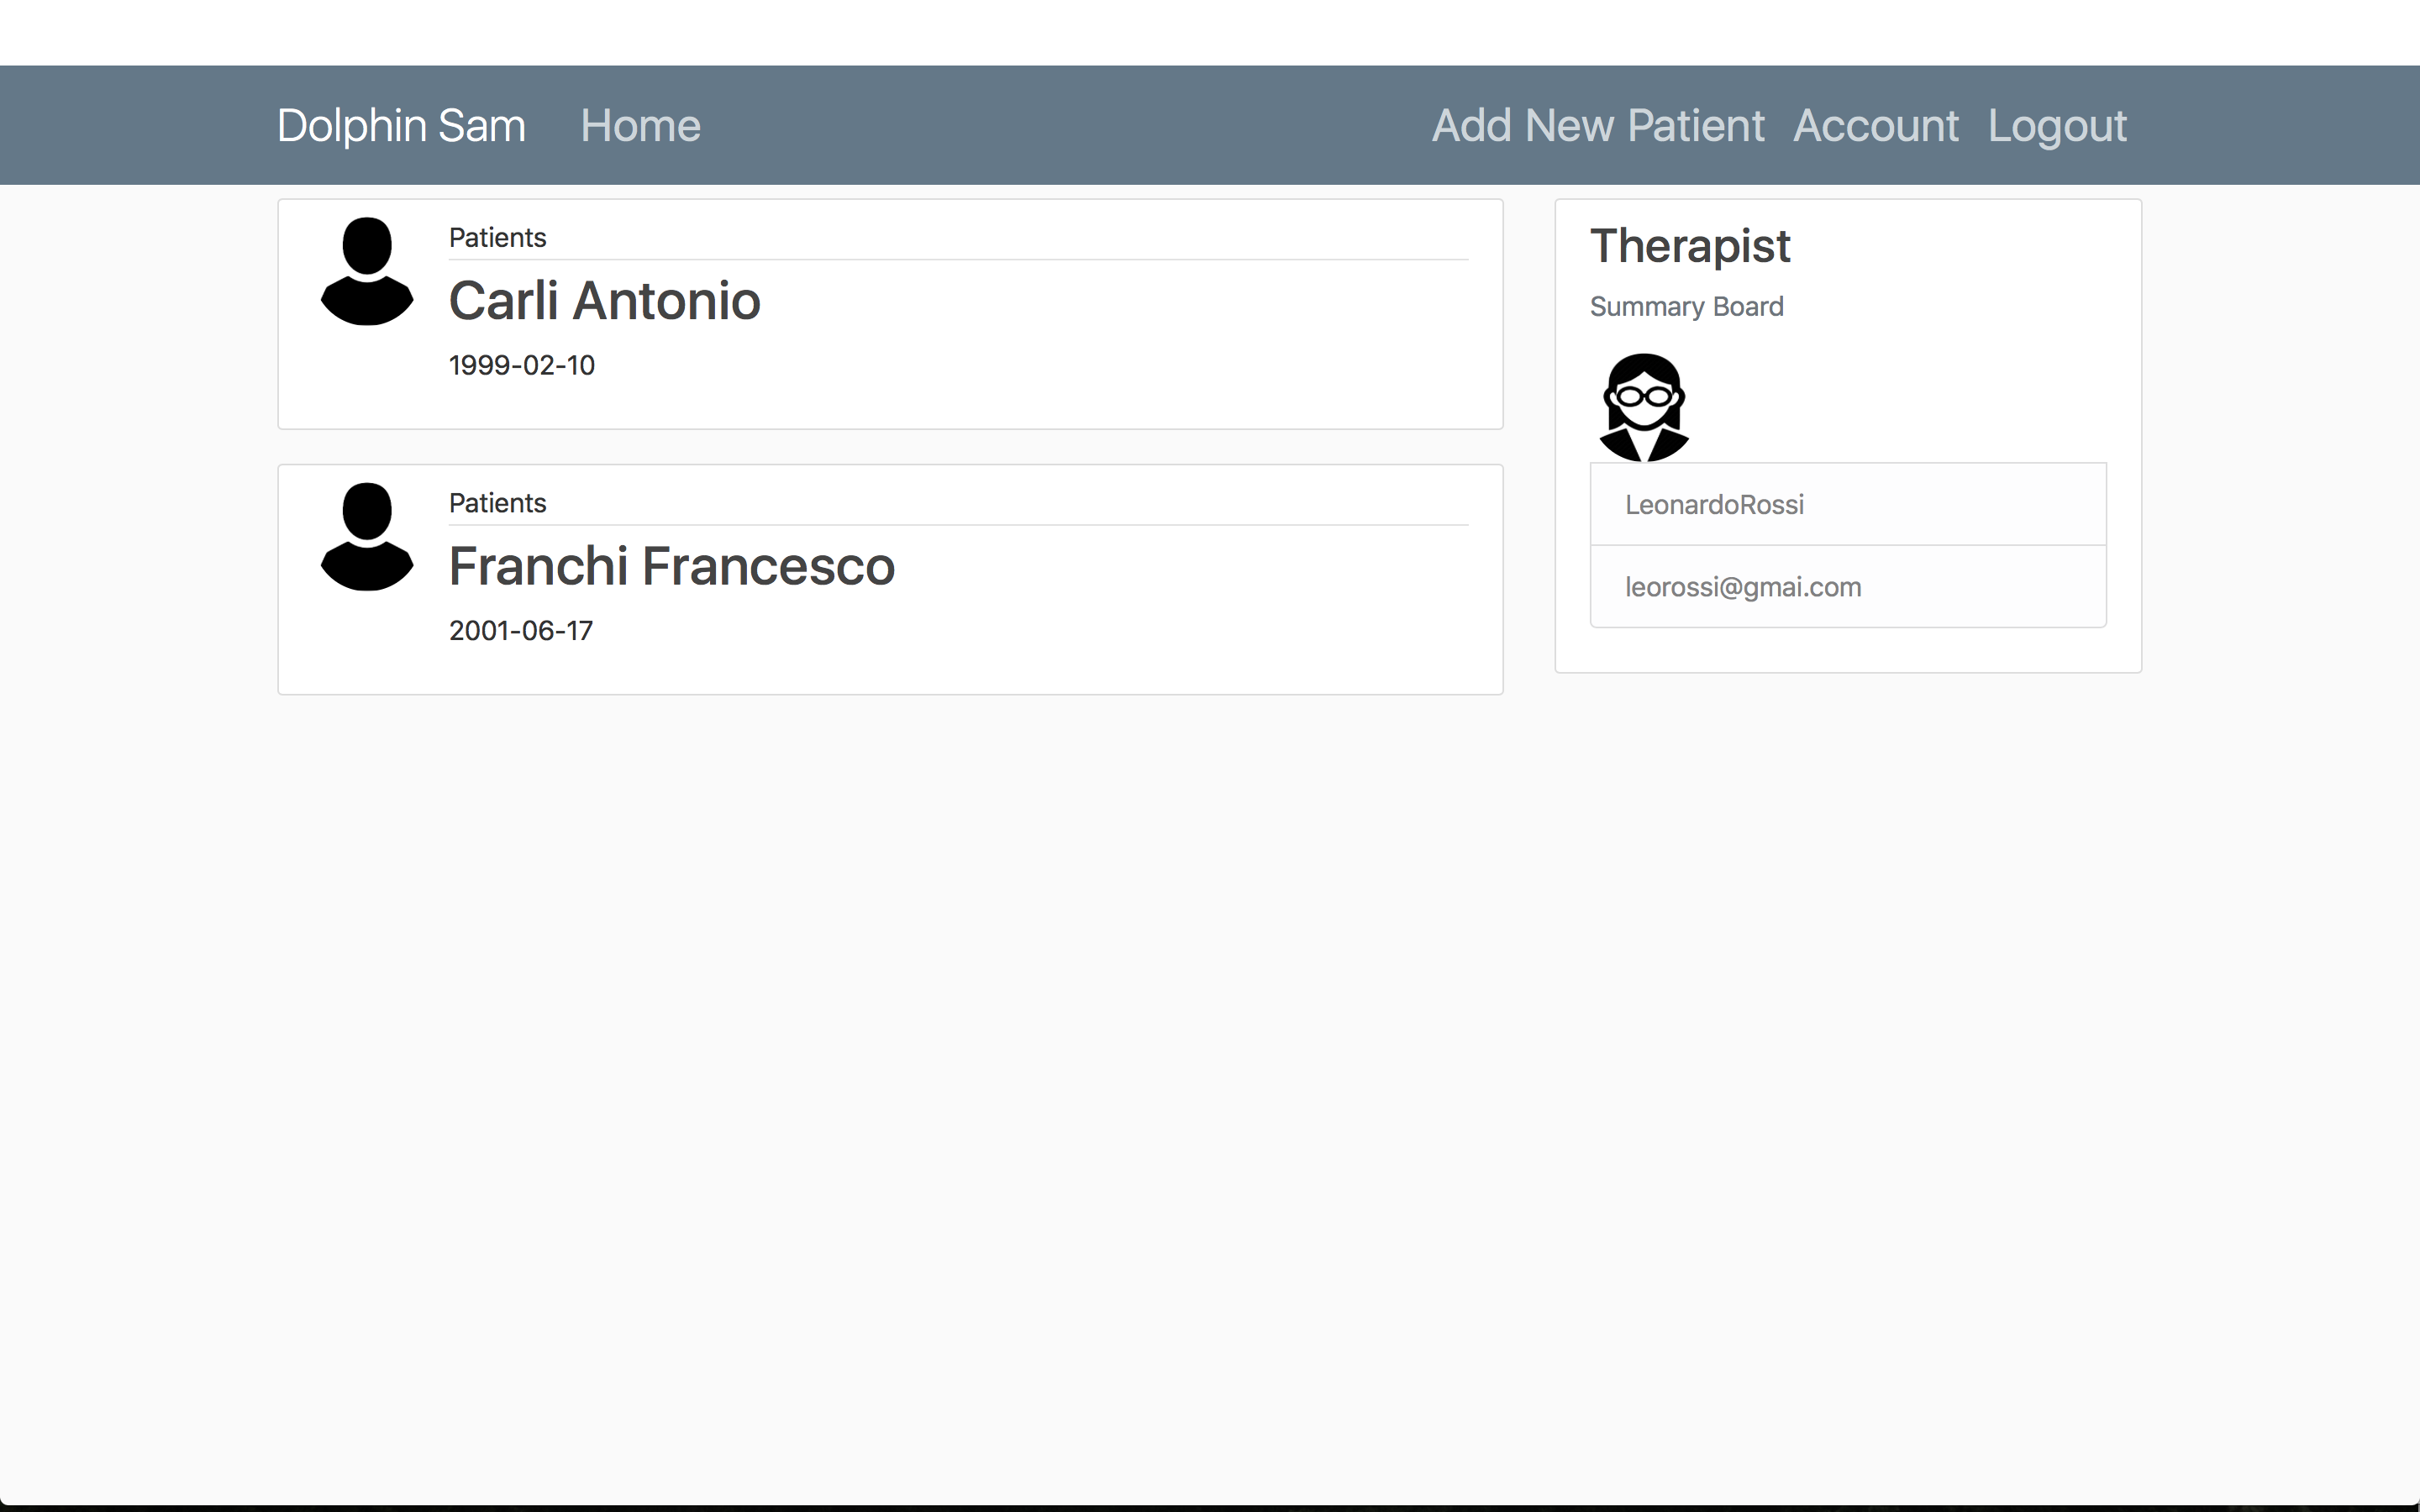
\includegraphics[width=\textwidth]{images/UX/website/4-patientsList}
	\caption{Therapist's personal home page}
	\label{fig:webPatList}
\end{figure}
In Figure \ref{fig:webPatList} is represented the website's personal page of the therapist that will be shown after a successful login authentication. Here he/she can see all his/her patients' records (note that a therapist can only manage and access records about his/her own patients), choose to add a new patient by pressing the "Add New Patient" button, edit his/her account by clicking the "Account" button and logout via the "Logout" button.

\begin{figure}[h!]
	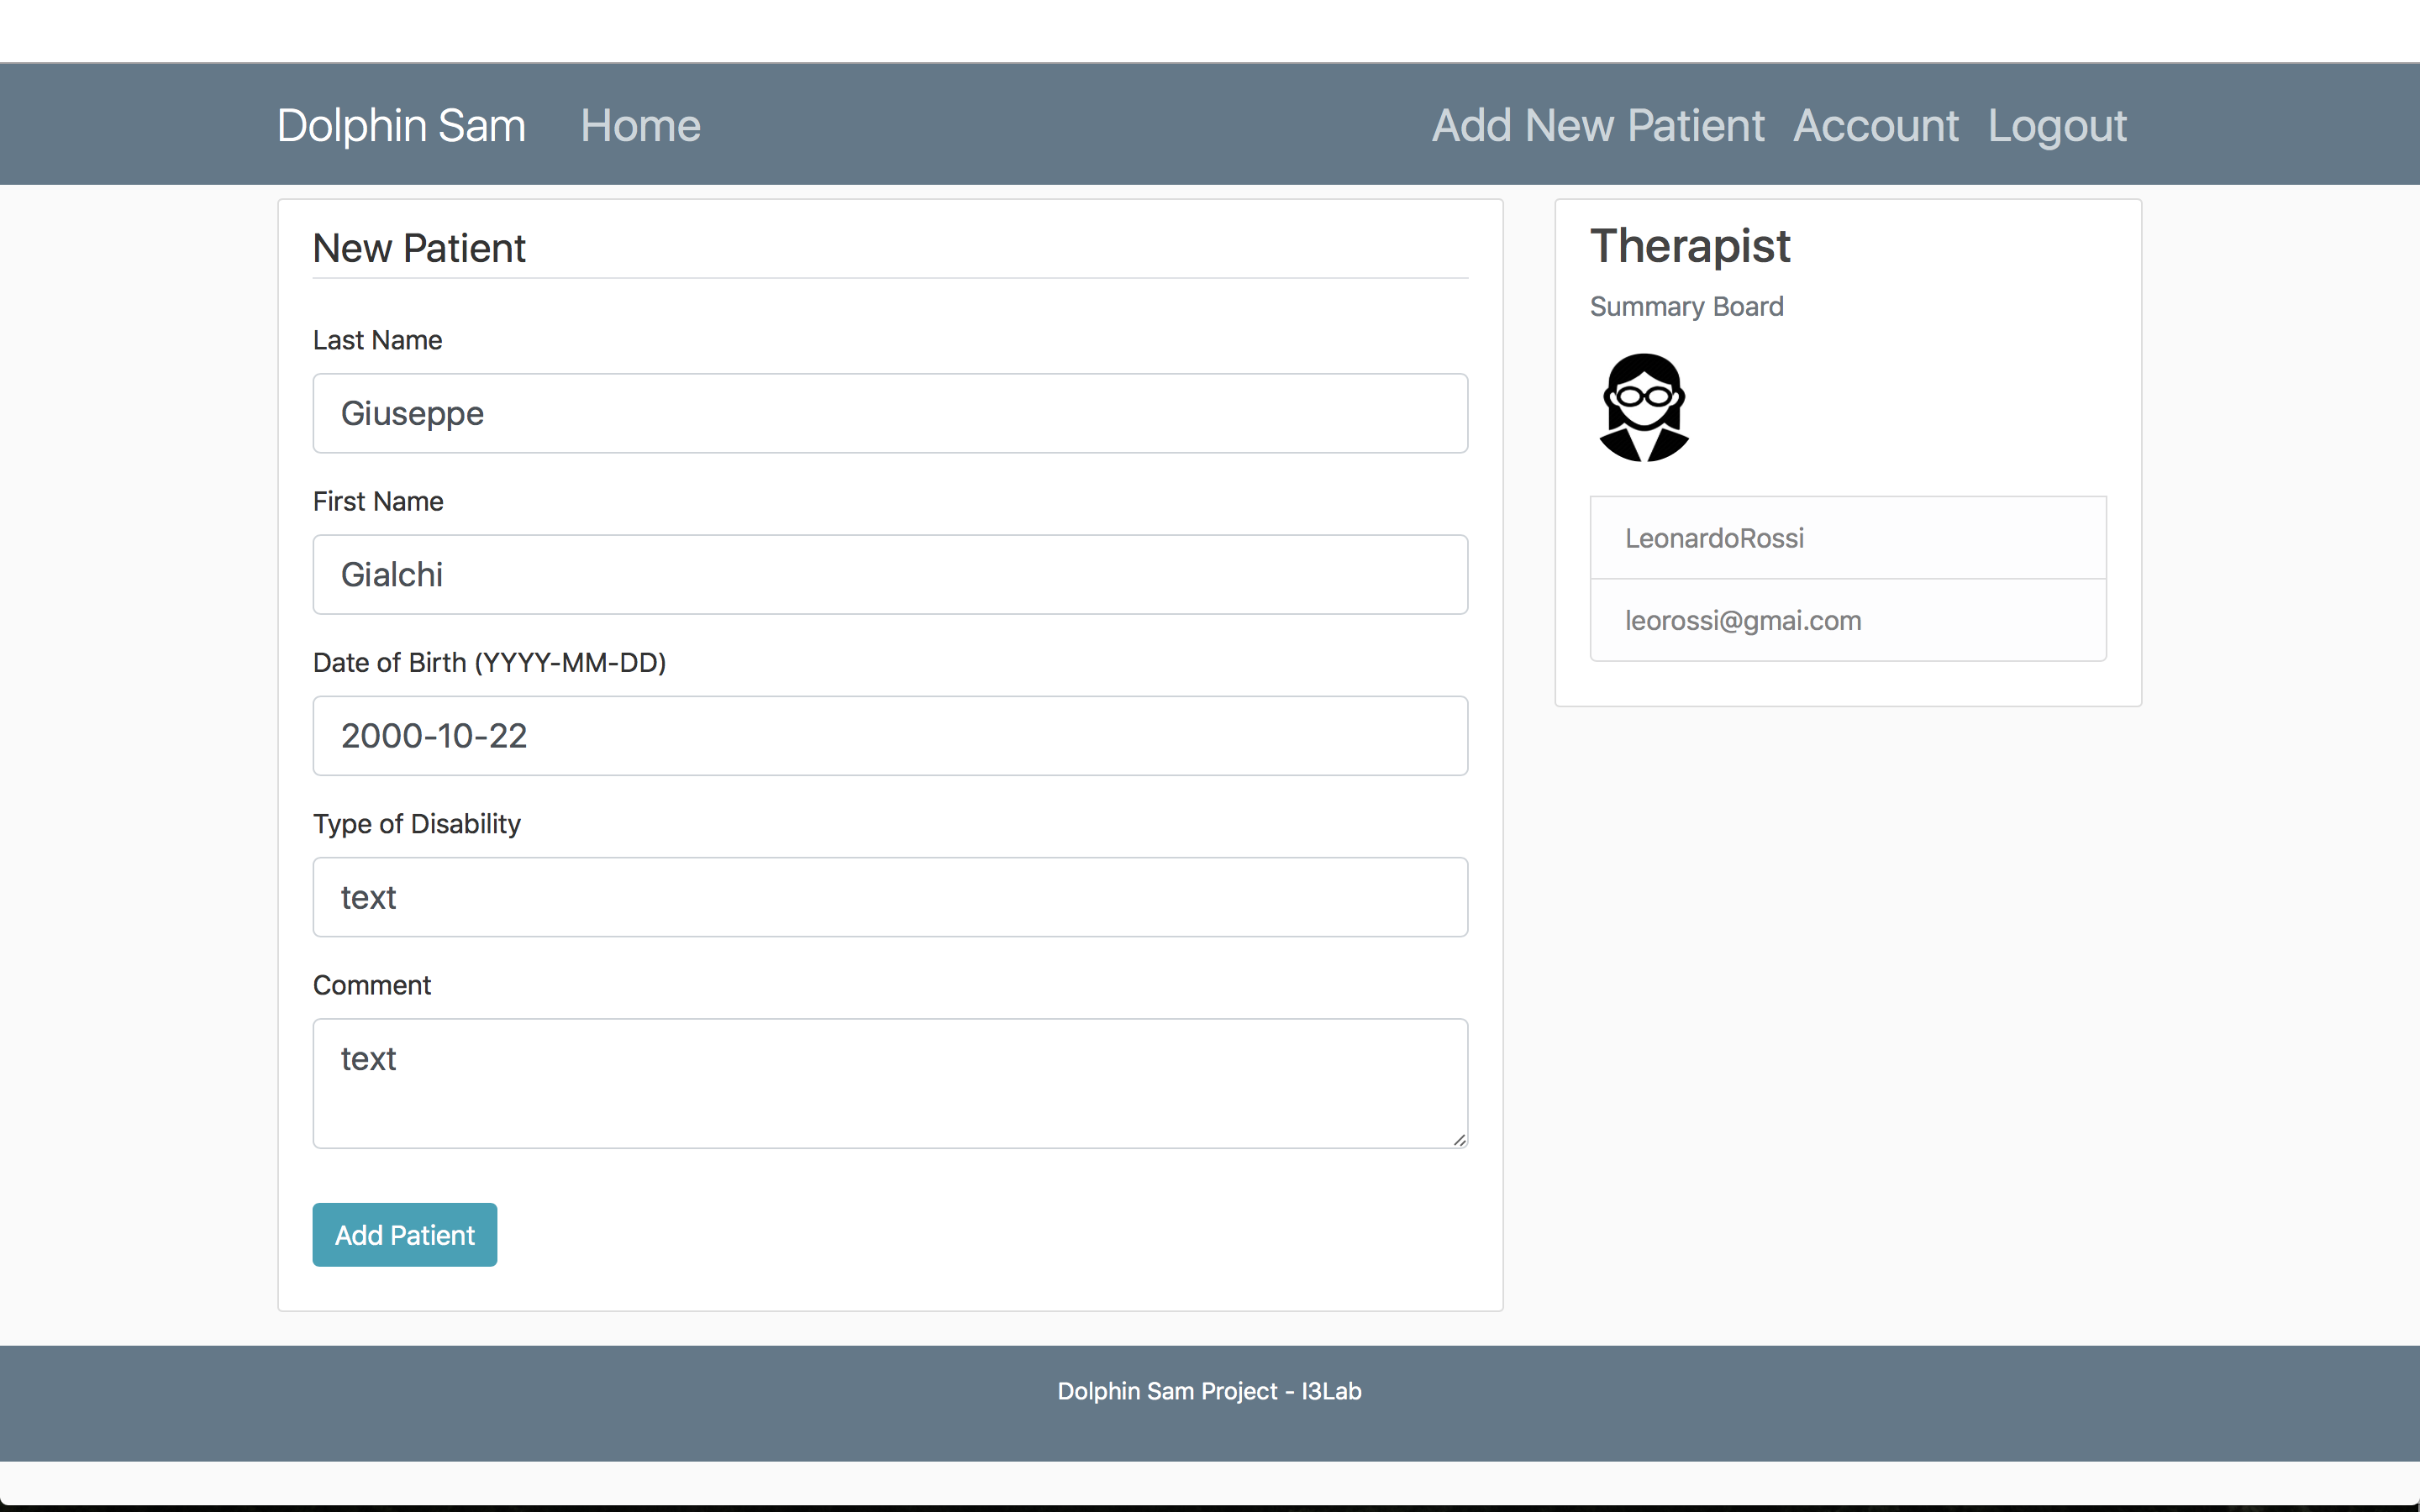
\includegraphics[width=\textwidth]{images/UX/website/6-addNewPatient}
	\caption{Add a new patient form}
	\label{fig:webAddPat}
\end{figure}
\pagebreak
In Figure  \ref{fig:webAddPat} is represented the form that will be used to collect the patient's information during the registration process brought by the therapist. When completed the new patient's record will be made persistent and added to the therapist's list of patients by clicking on the "Add Patient" button below.
\begin{figure}[h]
	\centering
	\begin{minipage}[b]{0.4\textwidth}
		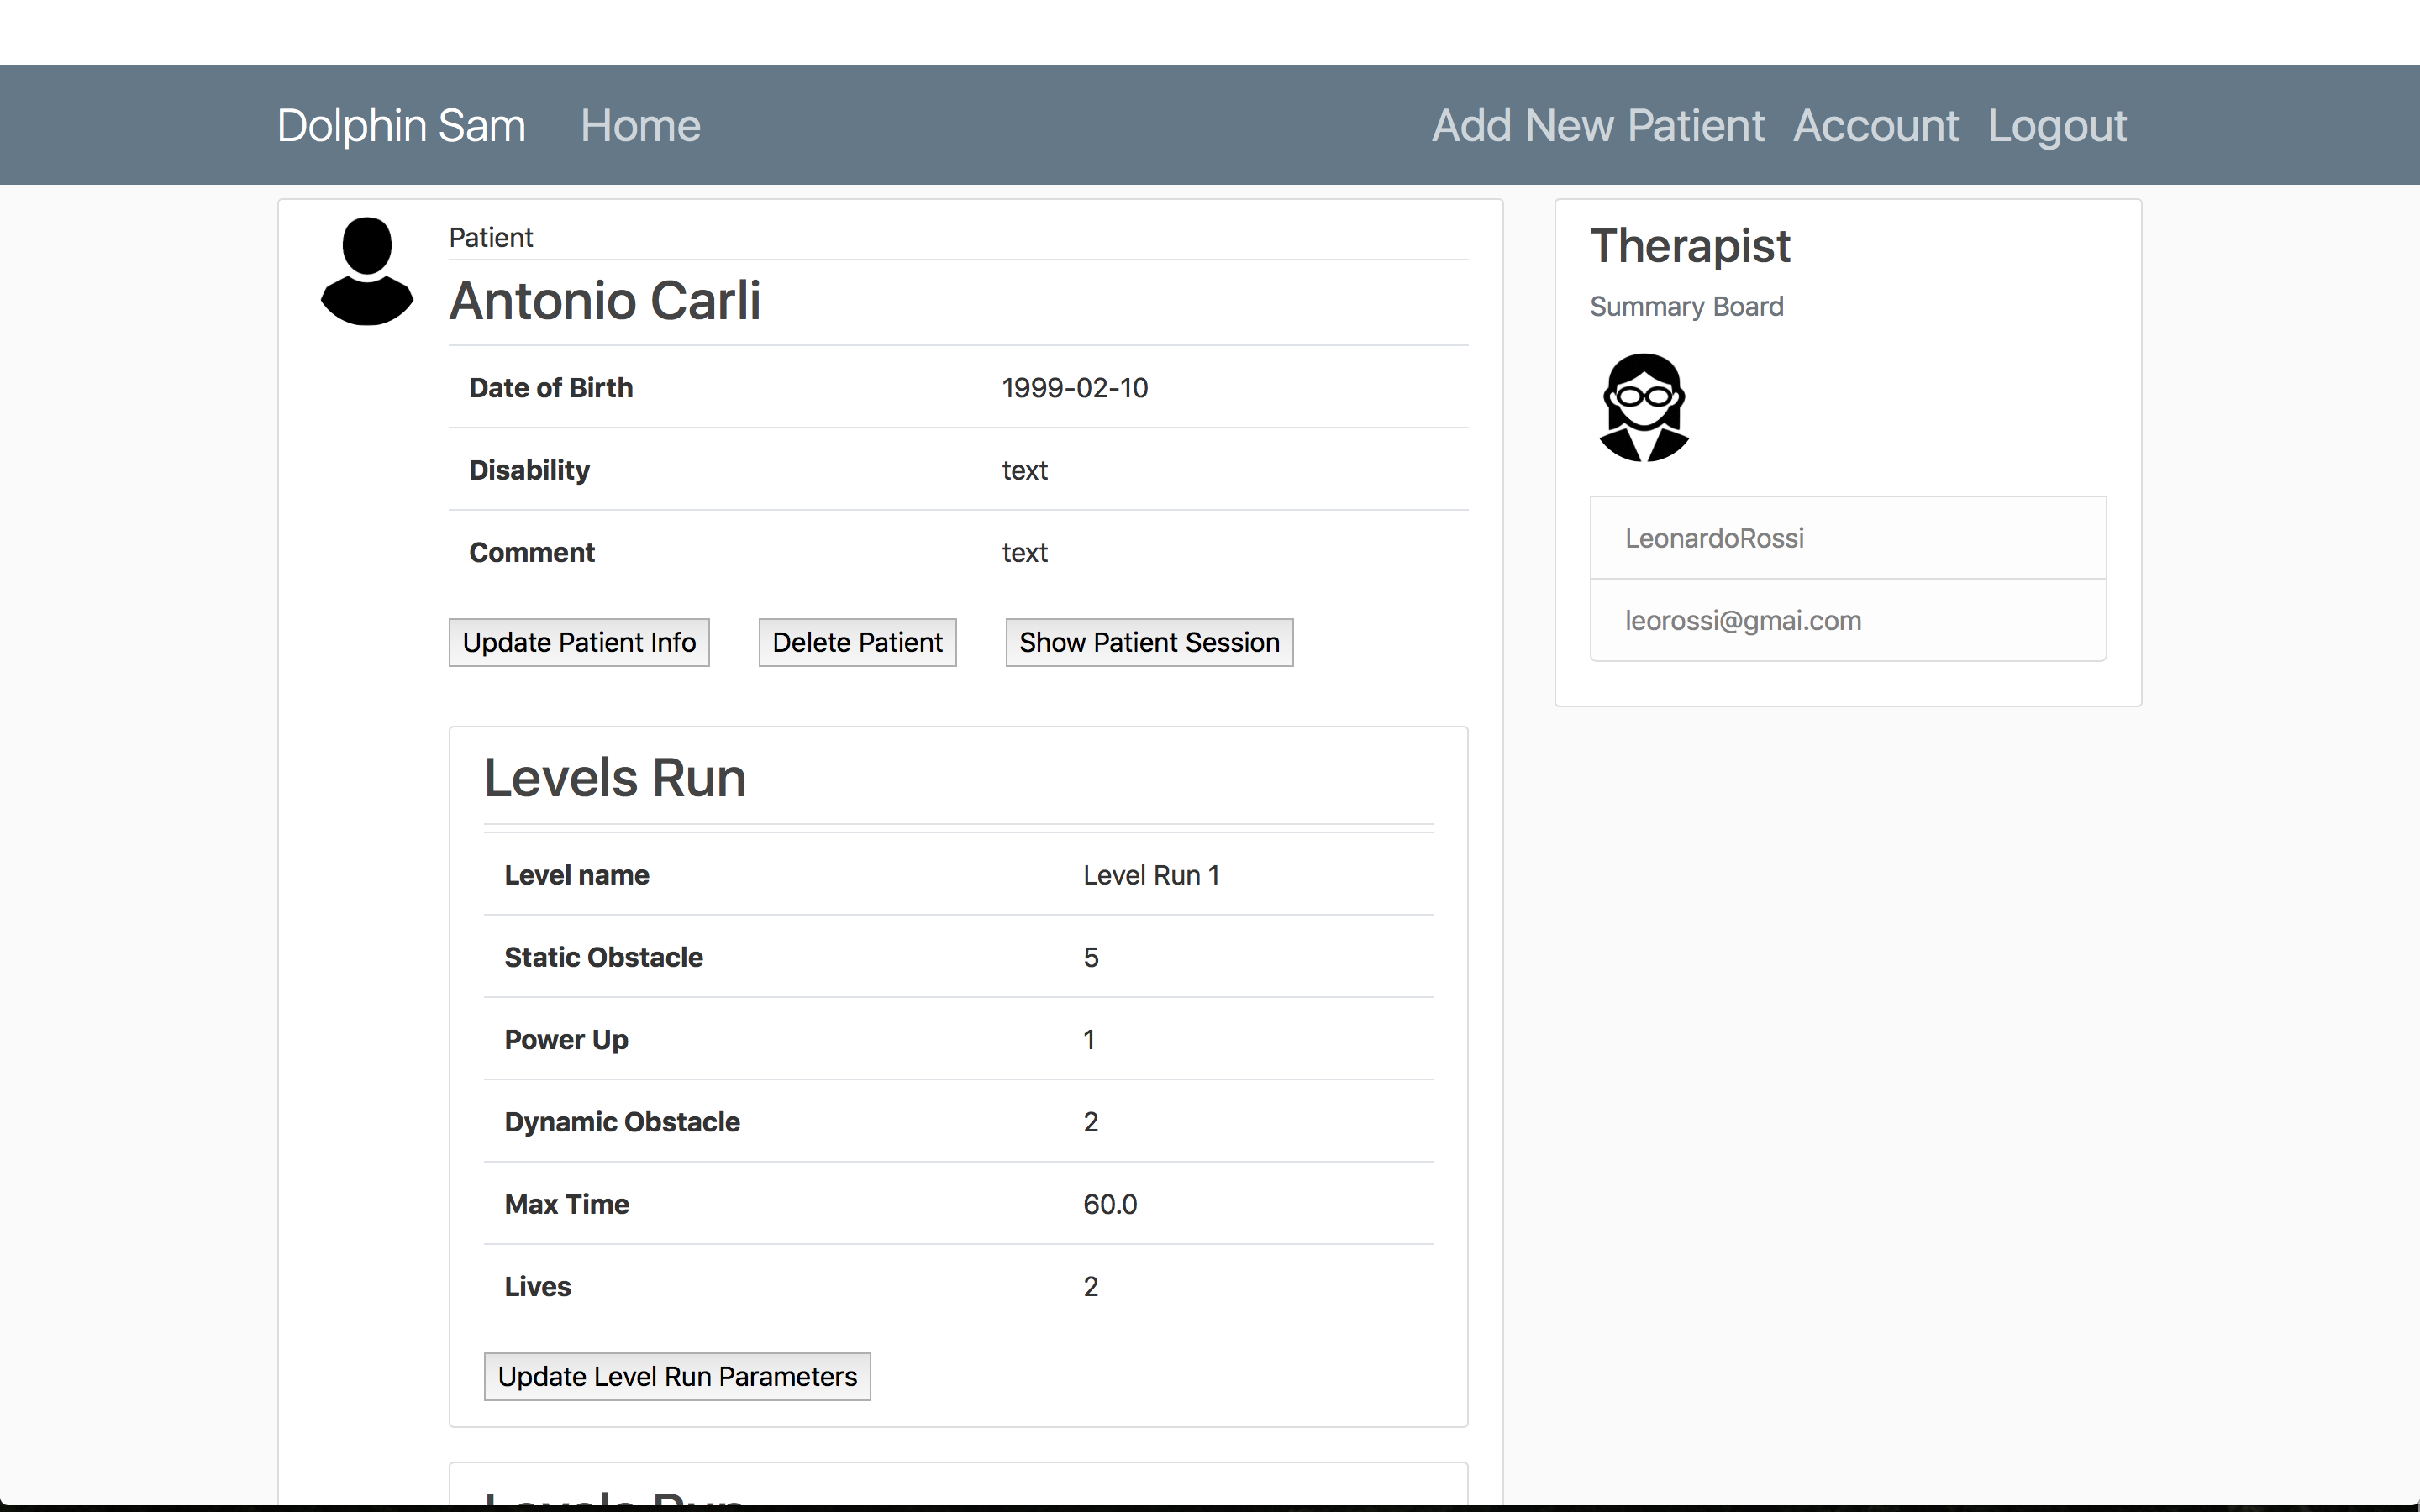
\includegraphics[width=\textwidth]{images/UX/website/7-detailPatient}
		\caption{Patient's parameters for the Run activity}
		\label{fig:webPatPar1}
	\end{minipage}
	\hfill
	\begin{minipage}[b]{0.4\textwidth}
		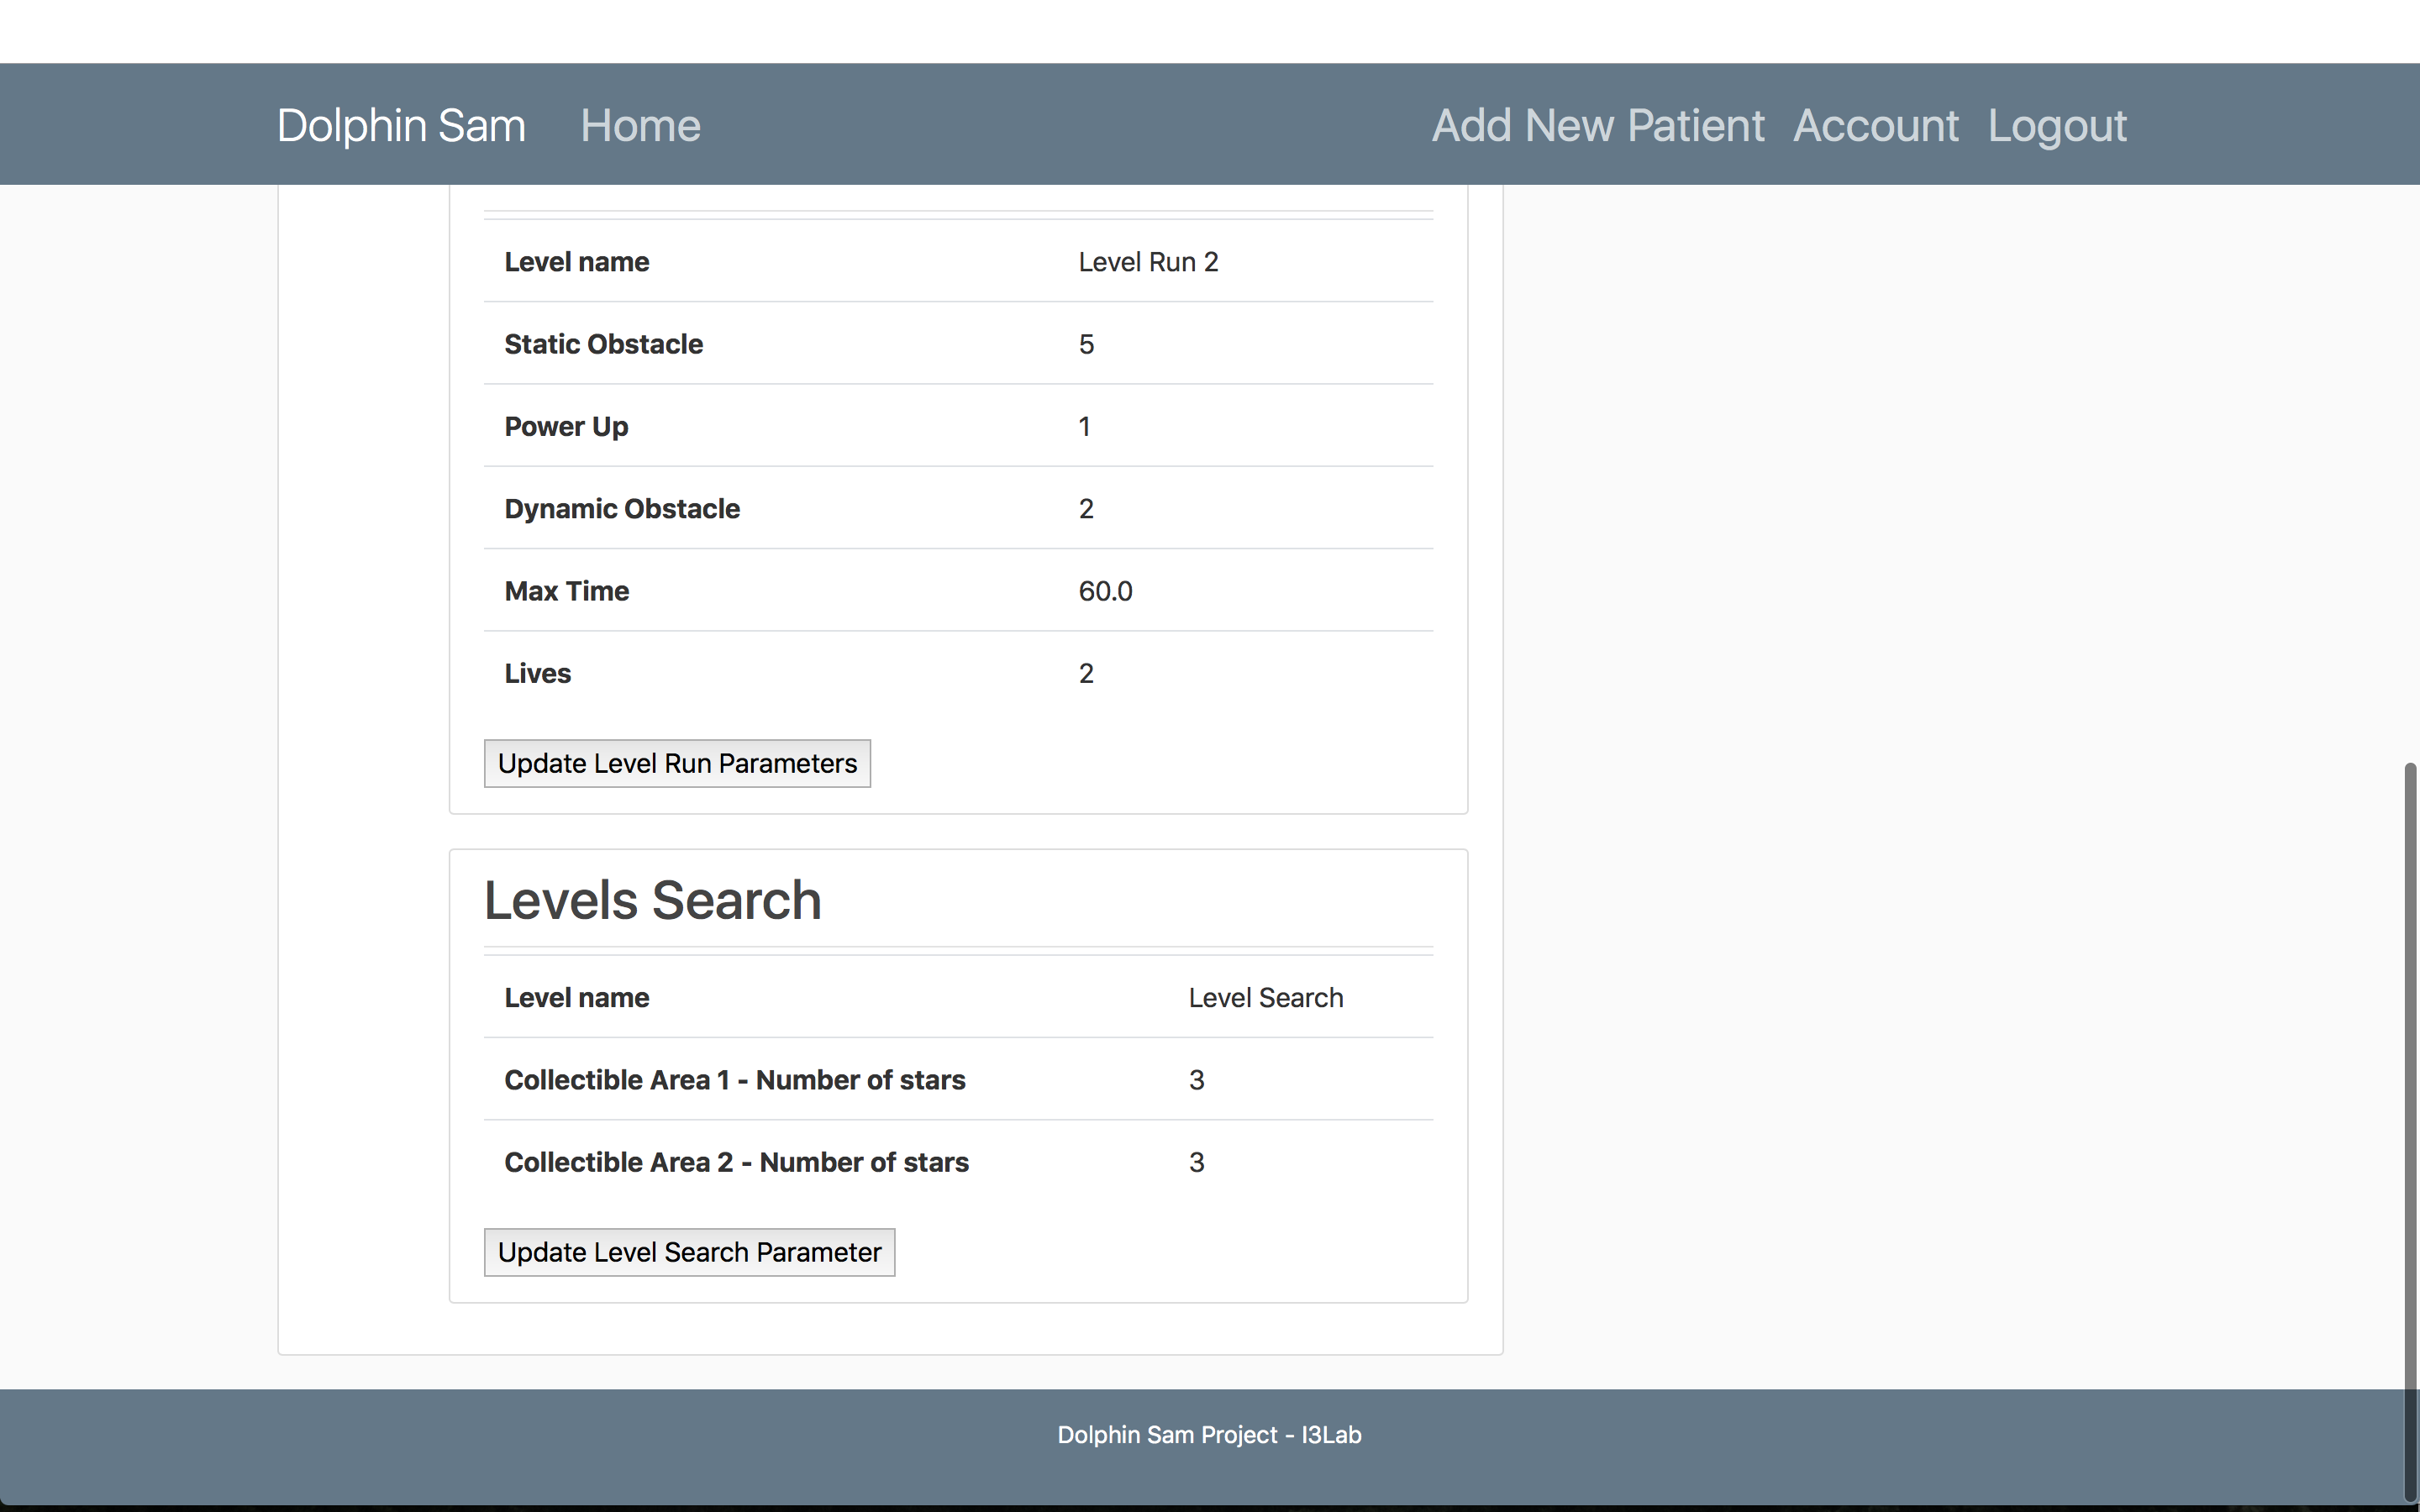
\includegraphics[width=\textwidth]{images/UX/website/8-detailPatient}
		\caption{Patient's parameters for the Search activity}
		\label{fig:webPatPar2}
	\end{minipage}
\end{figure}

By selecting a patient from the list (Figure  \ref{fig:webPatList})  the therapist is redirected to the patient's details page (Figure \ref{fig:webPatPar1}, \ref{fig:webPatPar2}) which contains the patient's information and the parameters that will be used to set the different levels of difficulty for the various activities. Those parameters can be updated by selecting the respective "Update" button below in order to customize the activities for the specific patient starting from the next session.

%\begin{figure}[h]
%	\centering
%	\begin{minipage}[b]{0.4\textwidth}
%		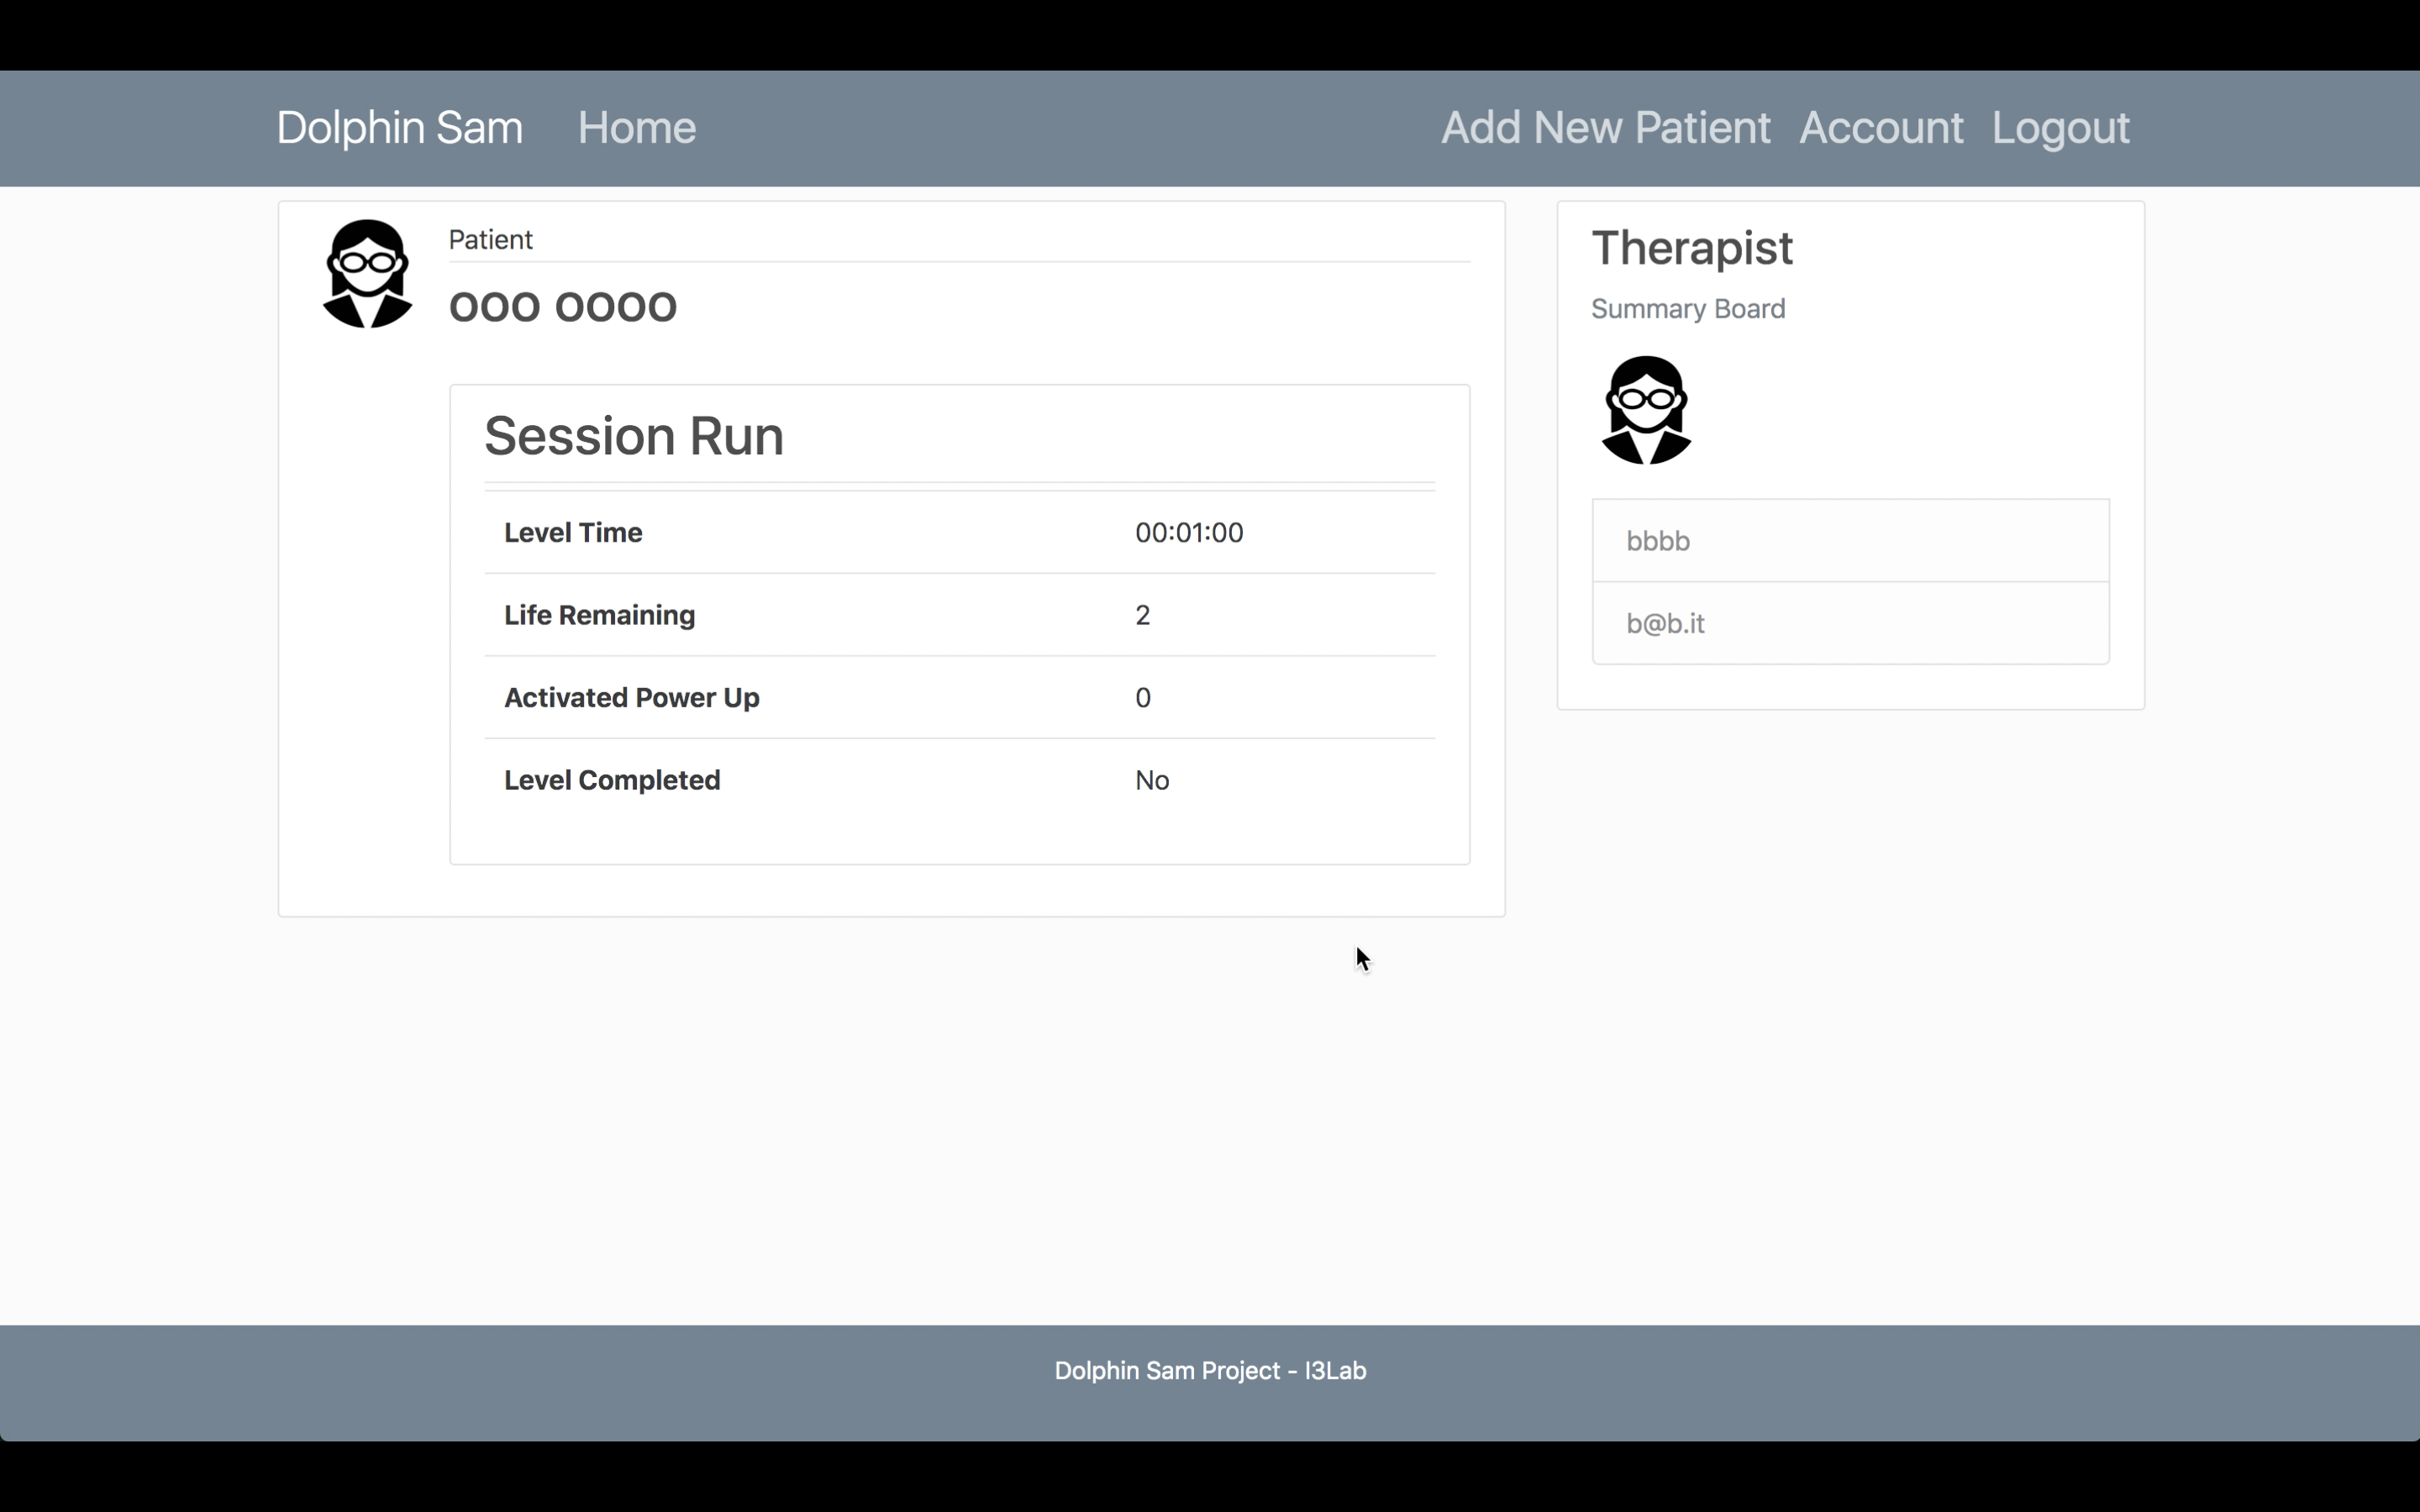
\includegraphics[width=\textwidth]{images/UX/website/11-runAnal}
%		\caption{Session data for Dolphin Run activity}
%		\label{fig:webAnalRun}
%	\end{minipage}
%	\hfill
%	\begin{minipage}[b]{0.4\textwidth}
%		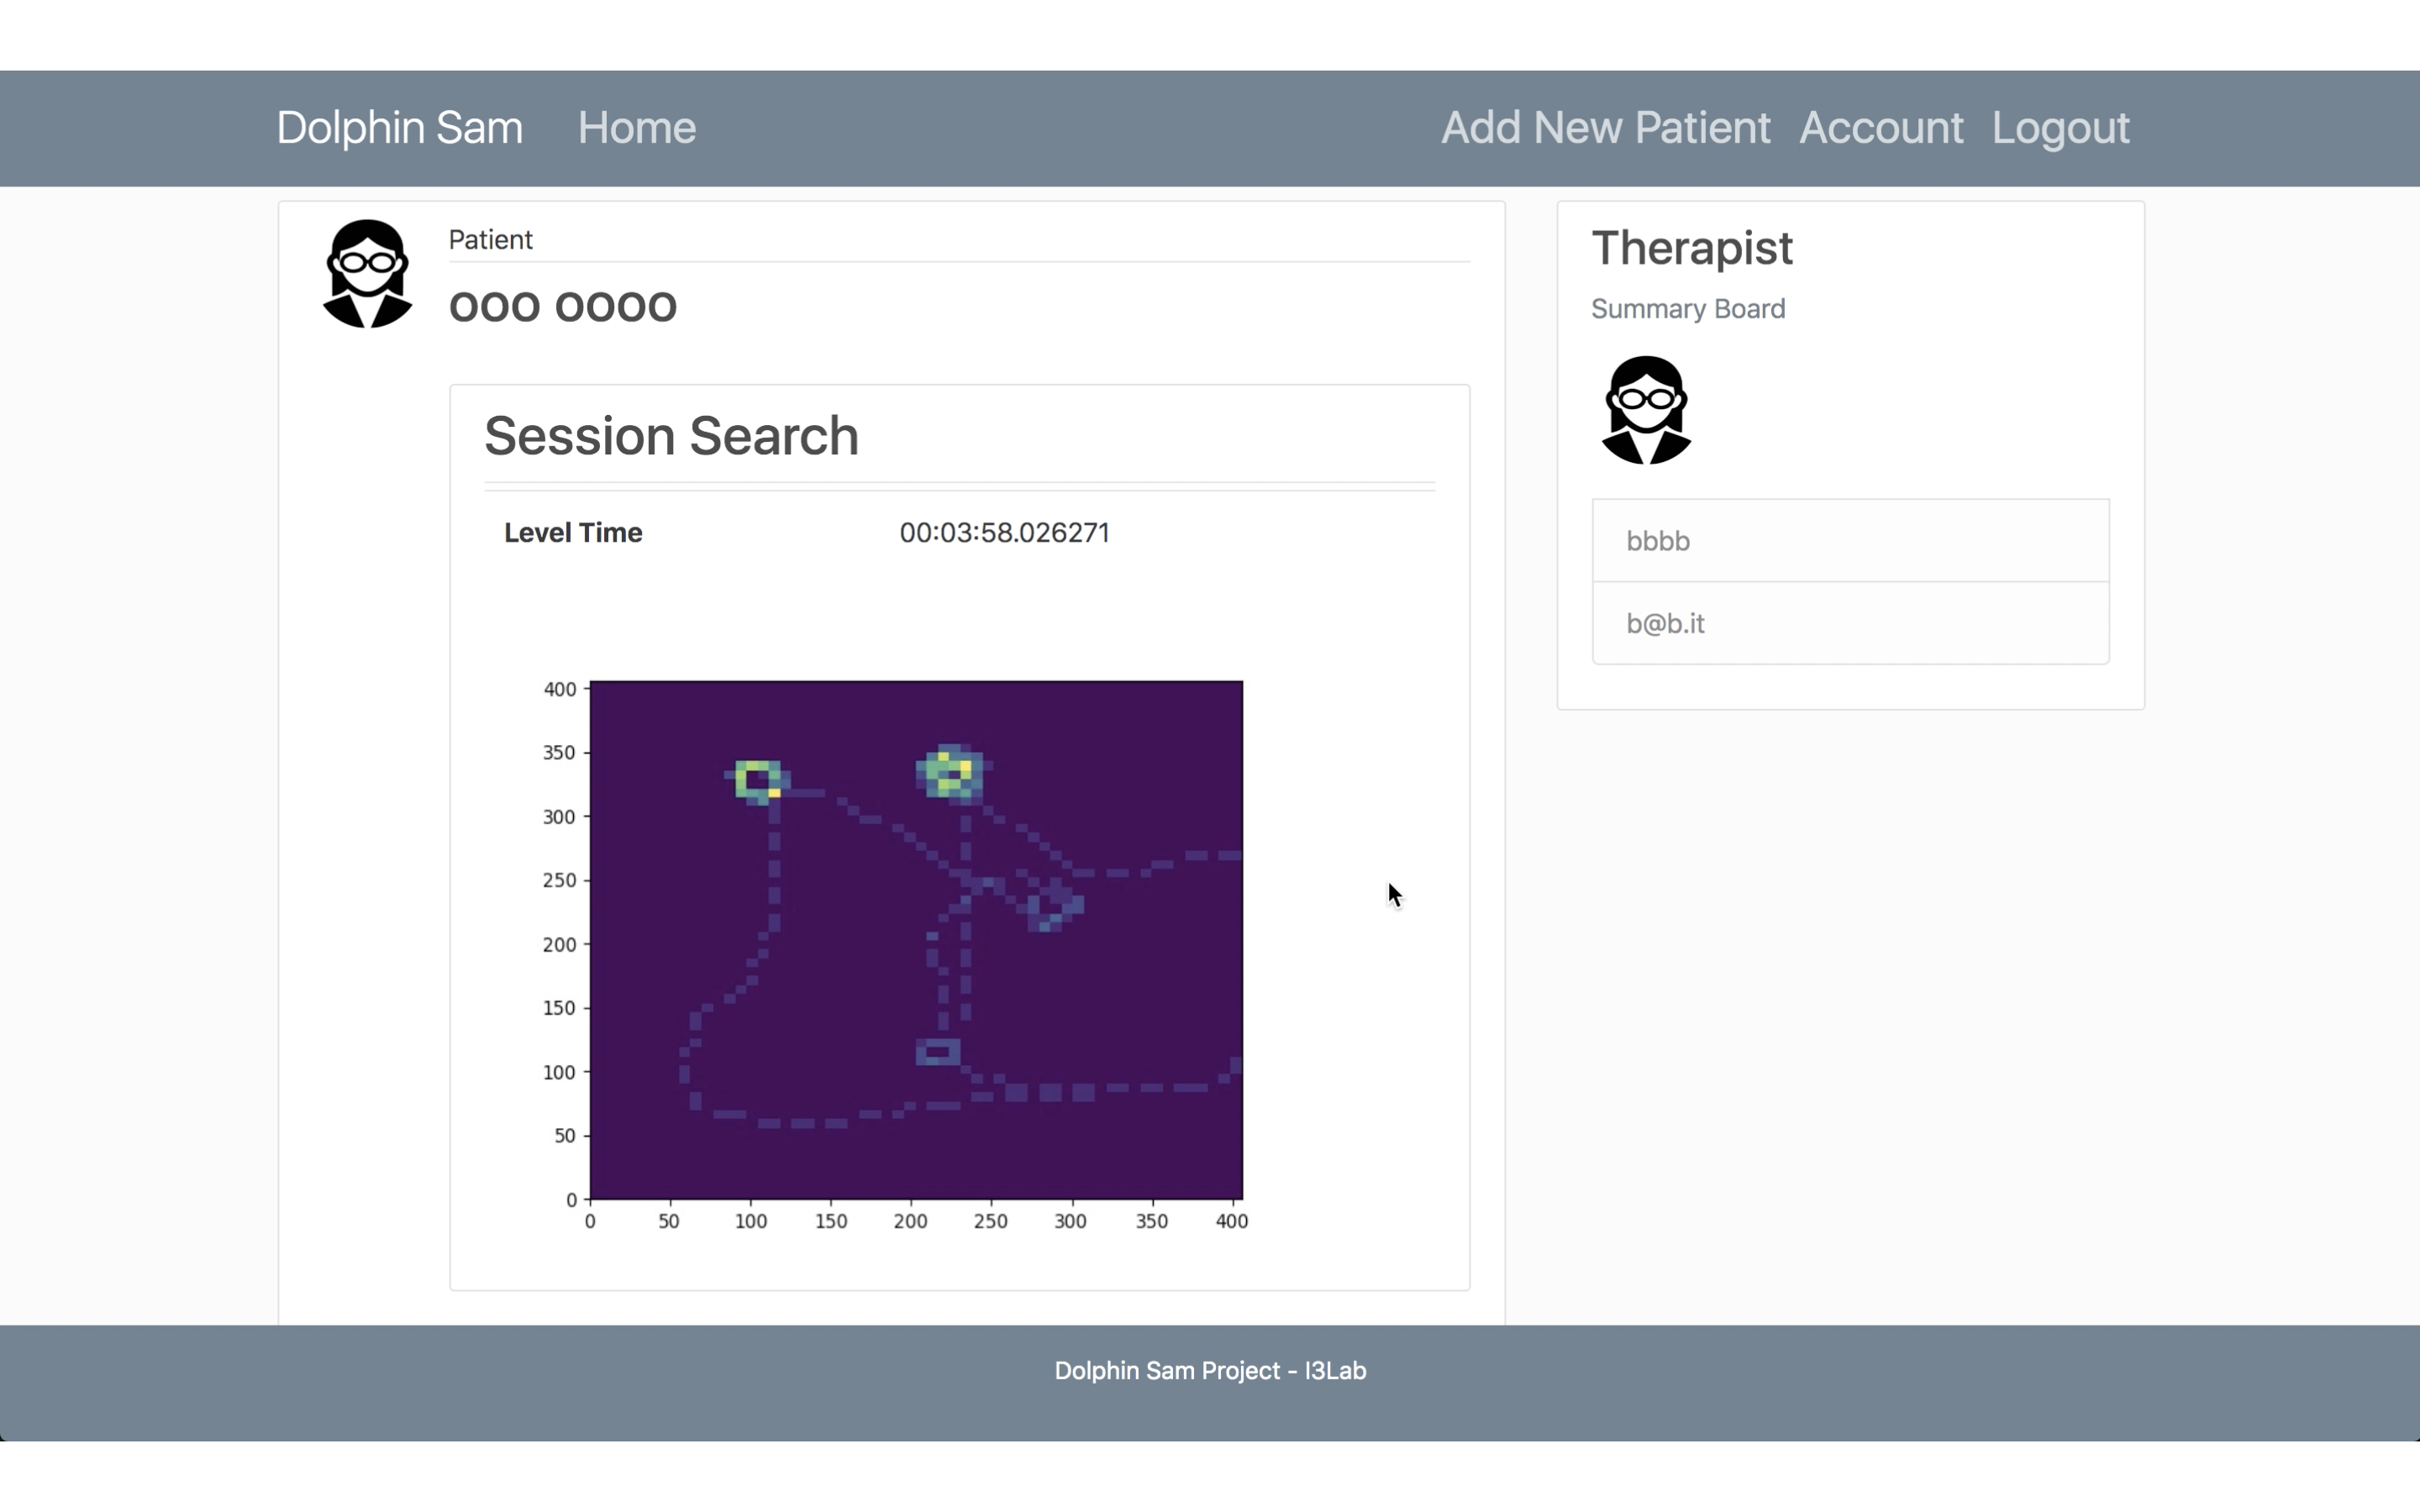
\includegraphics[width=\textwidth]{images/UX/website/12-searchAnal}
%		\caption{Session data for Dolphin Search activity}
%		\label{fig:webAnalSearch}
%	\end{minipage}
%\end{figure}

By clicking on the "Show Patient Session" button in a patient's detail page the therapist is able to see the data regarding all the session performed by the patient during the Dolphin Run activity (Figure \ref{fig:webAnalRun}) and the Dolphin Search activity (Figure \ref{fig:webAnalSearch}).



\subsection{Unity client}
\begin{figure}[h!]
	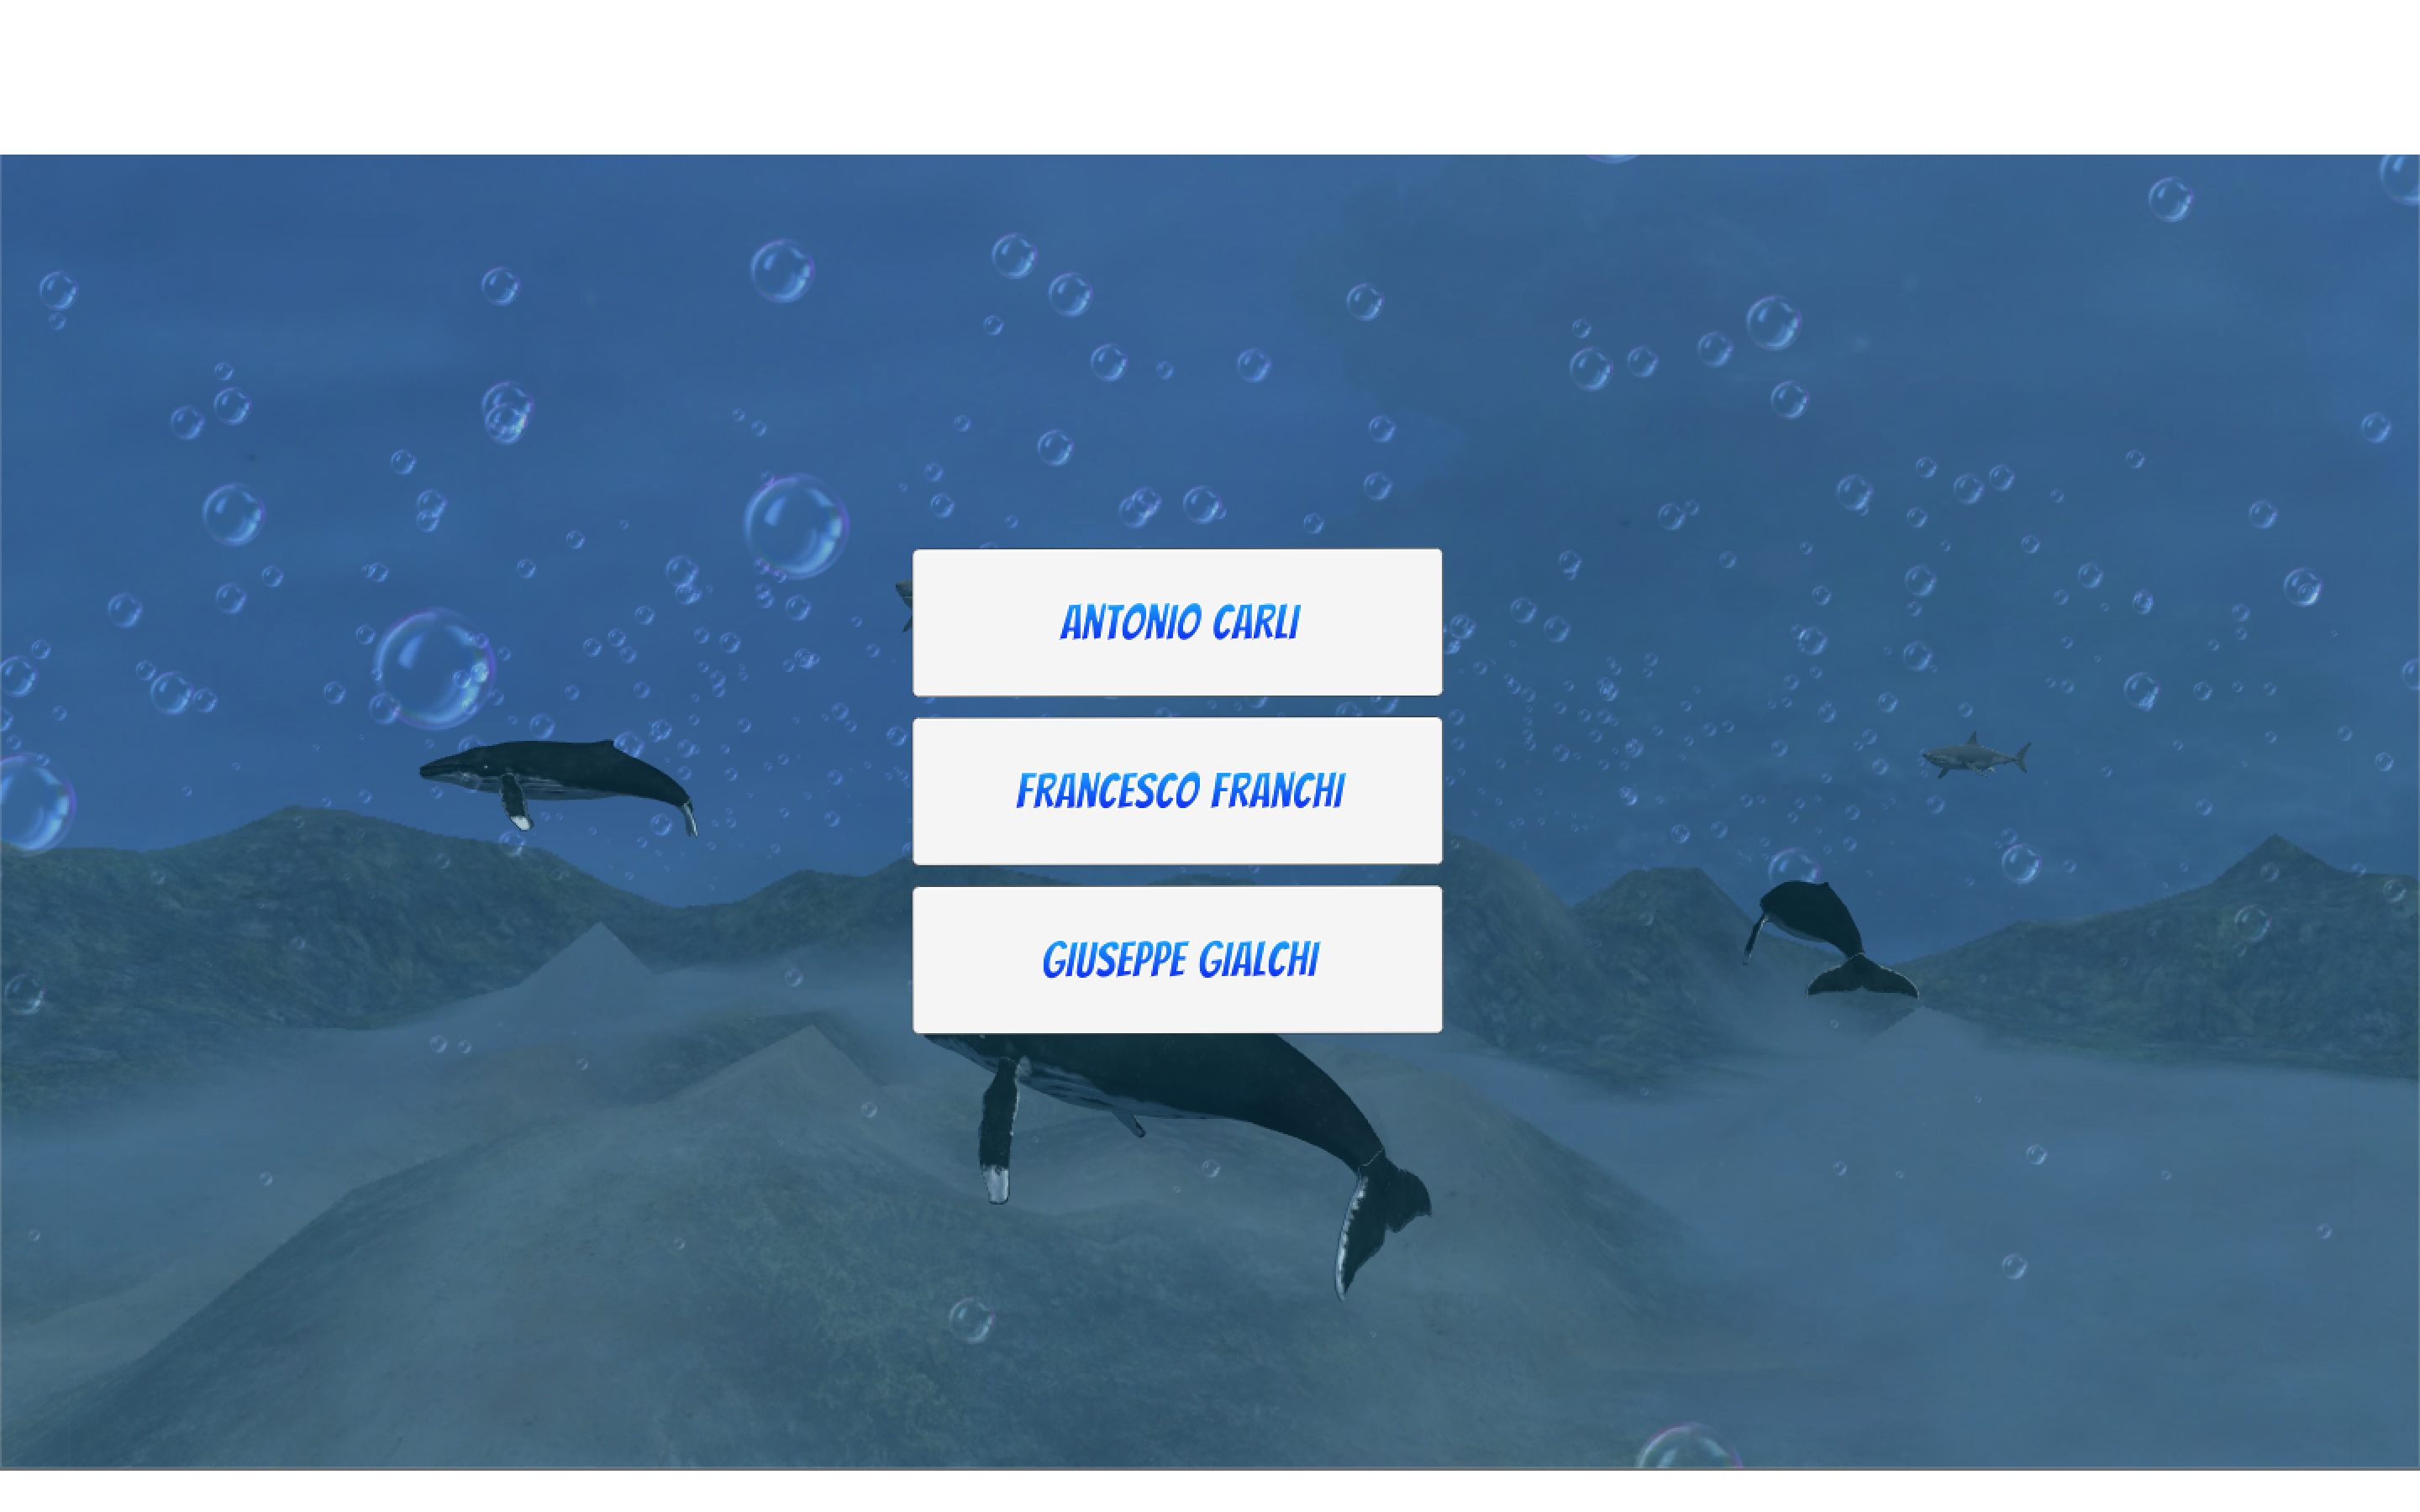
\includegraphics[width=\textwidth]{images/UX/unity/menu/3-patientList}
	\caption{Therapist's patient list}
	\label{fig:unityPatList}
\end{figure}
Once the game is started the therapist is logged in, his/her patients' list is shown (Figure \ref{fig:unityPatList}) and the patient that will perform the session has to be selected.
\begin{figure}[h]
	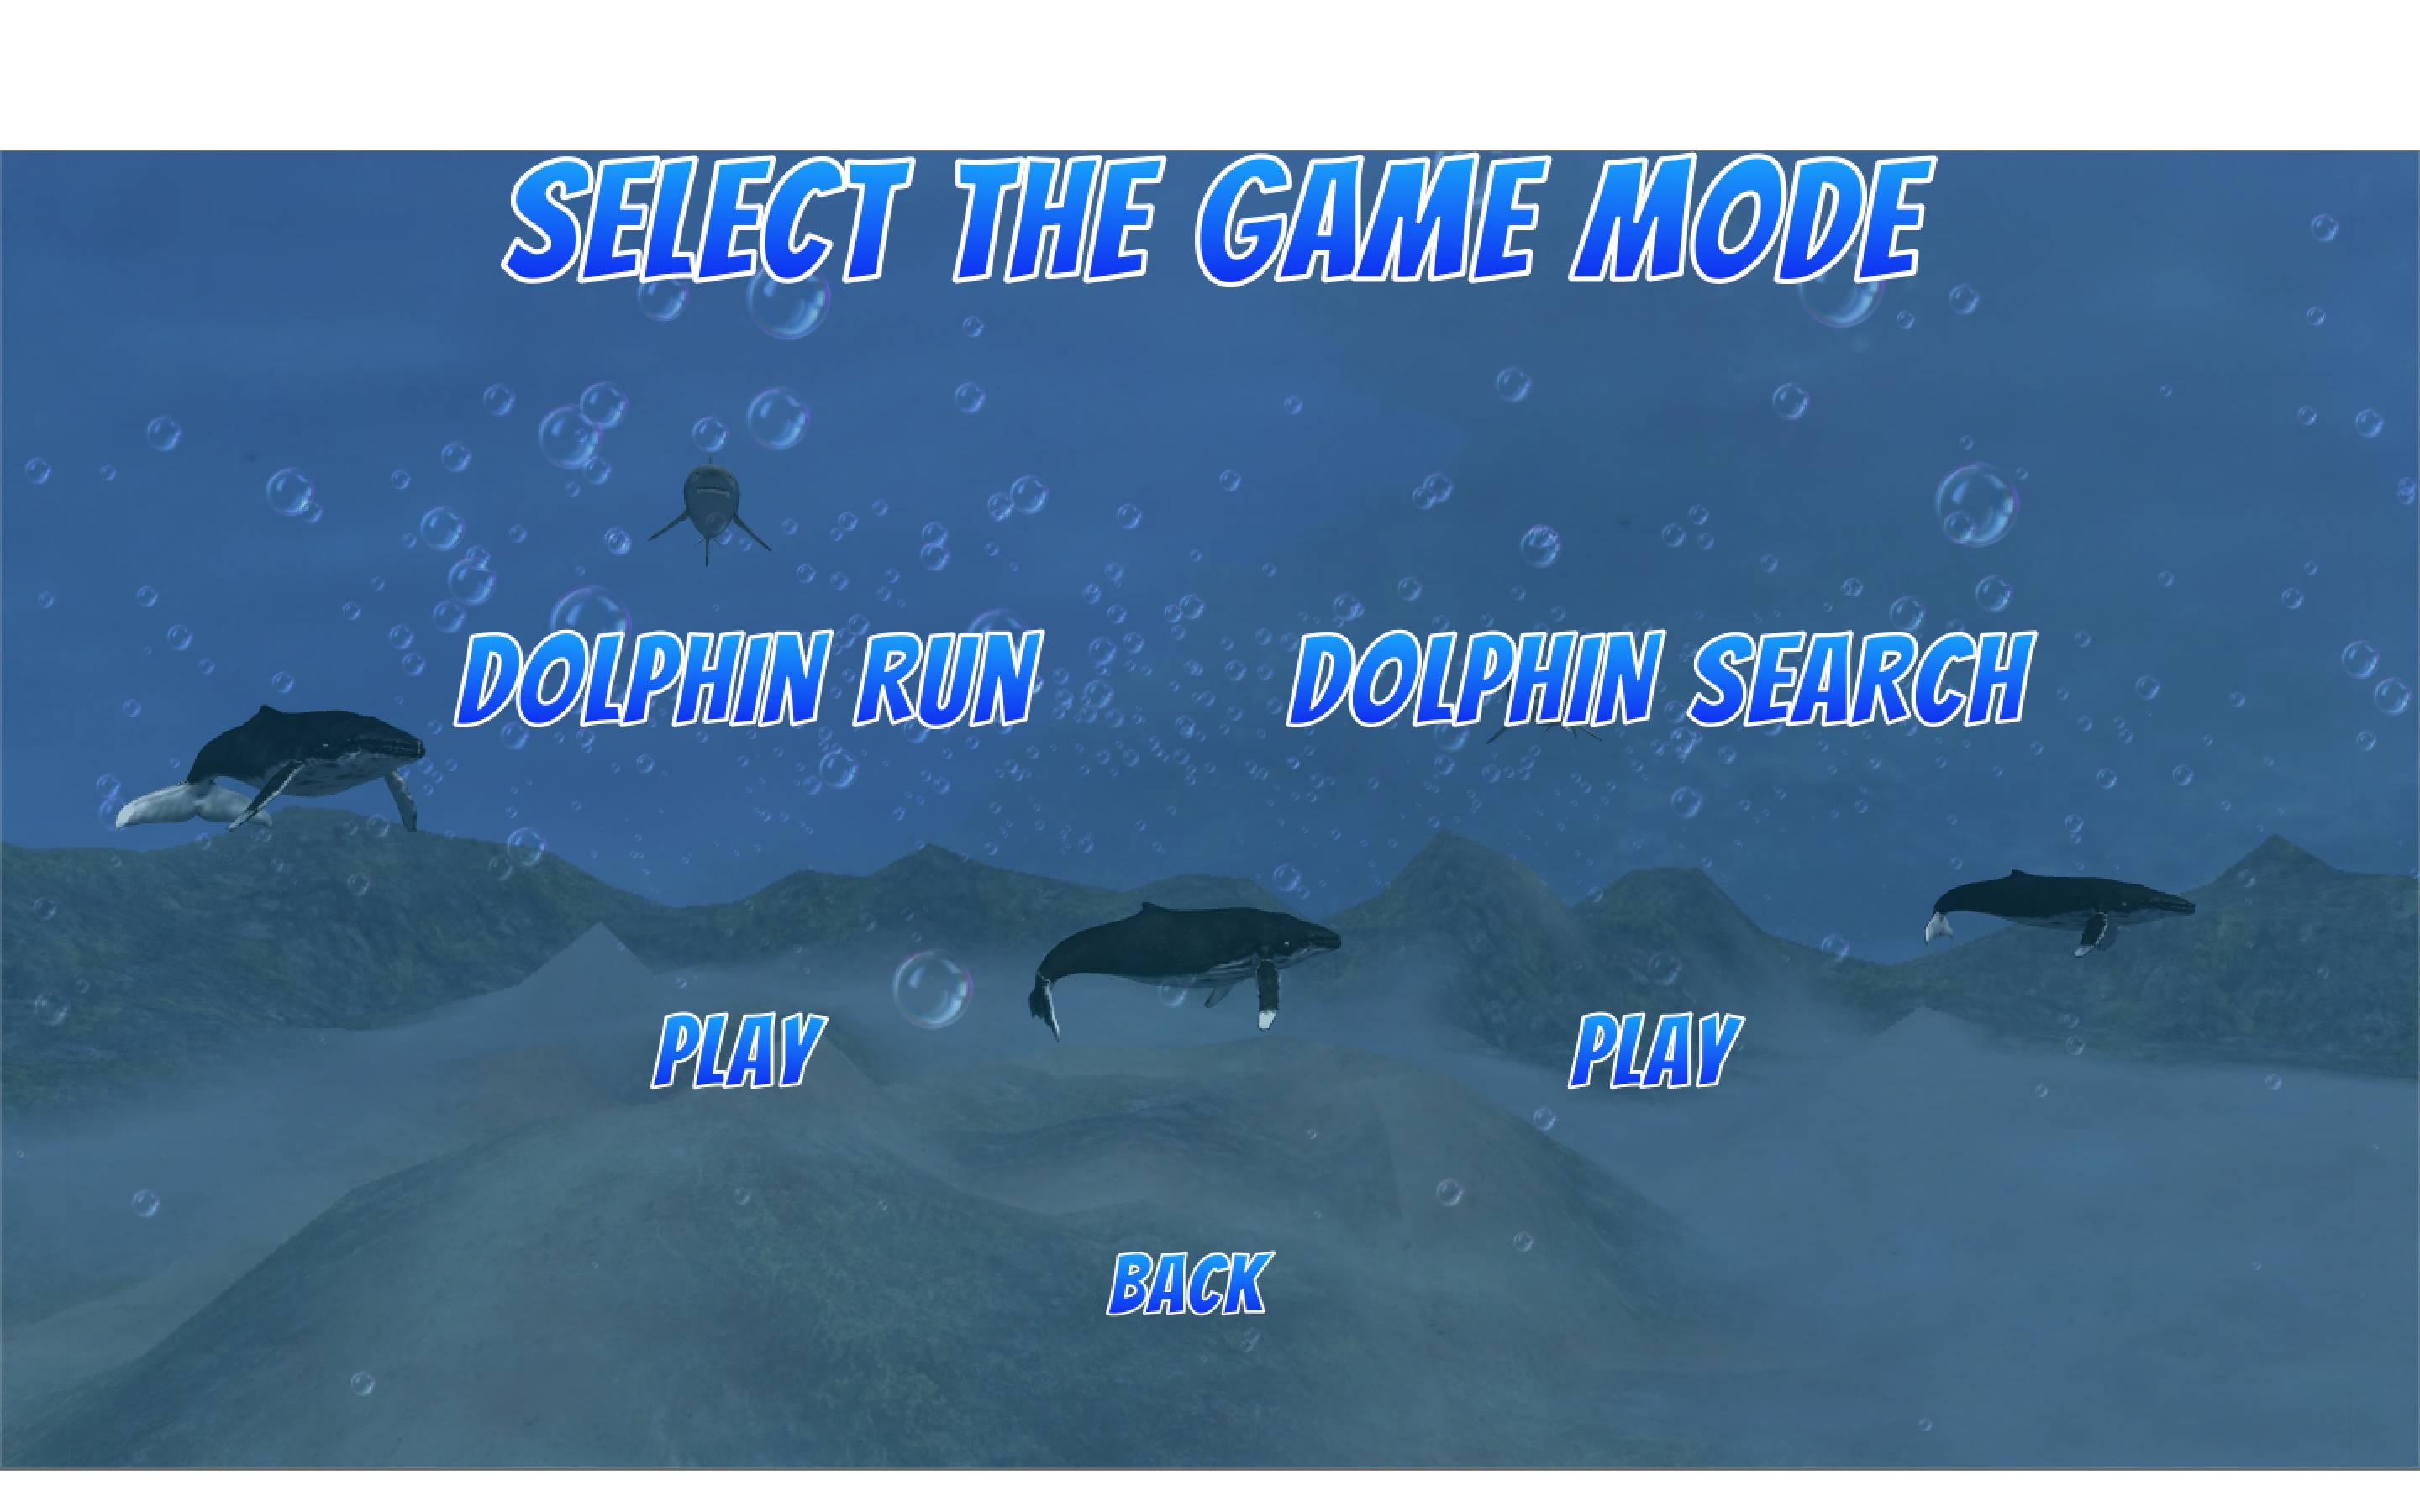
\includegraphics[width=\textwidth]{images/UX/unity/menu/4-modeSelection}
	\caption{Session's mode selection}
	\label{fig:unityModSel}
\end{figure}
After selecting a patient there will be asked to select which one of the activities (Dolphin run or Dolphin Search) will be played in the next session. (Figure \ref{fig:unityModSel}).
\begin{figure}[h]
	\centering
	\begin{minipage}[b]{0.4\textwidth}
		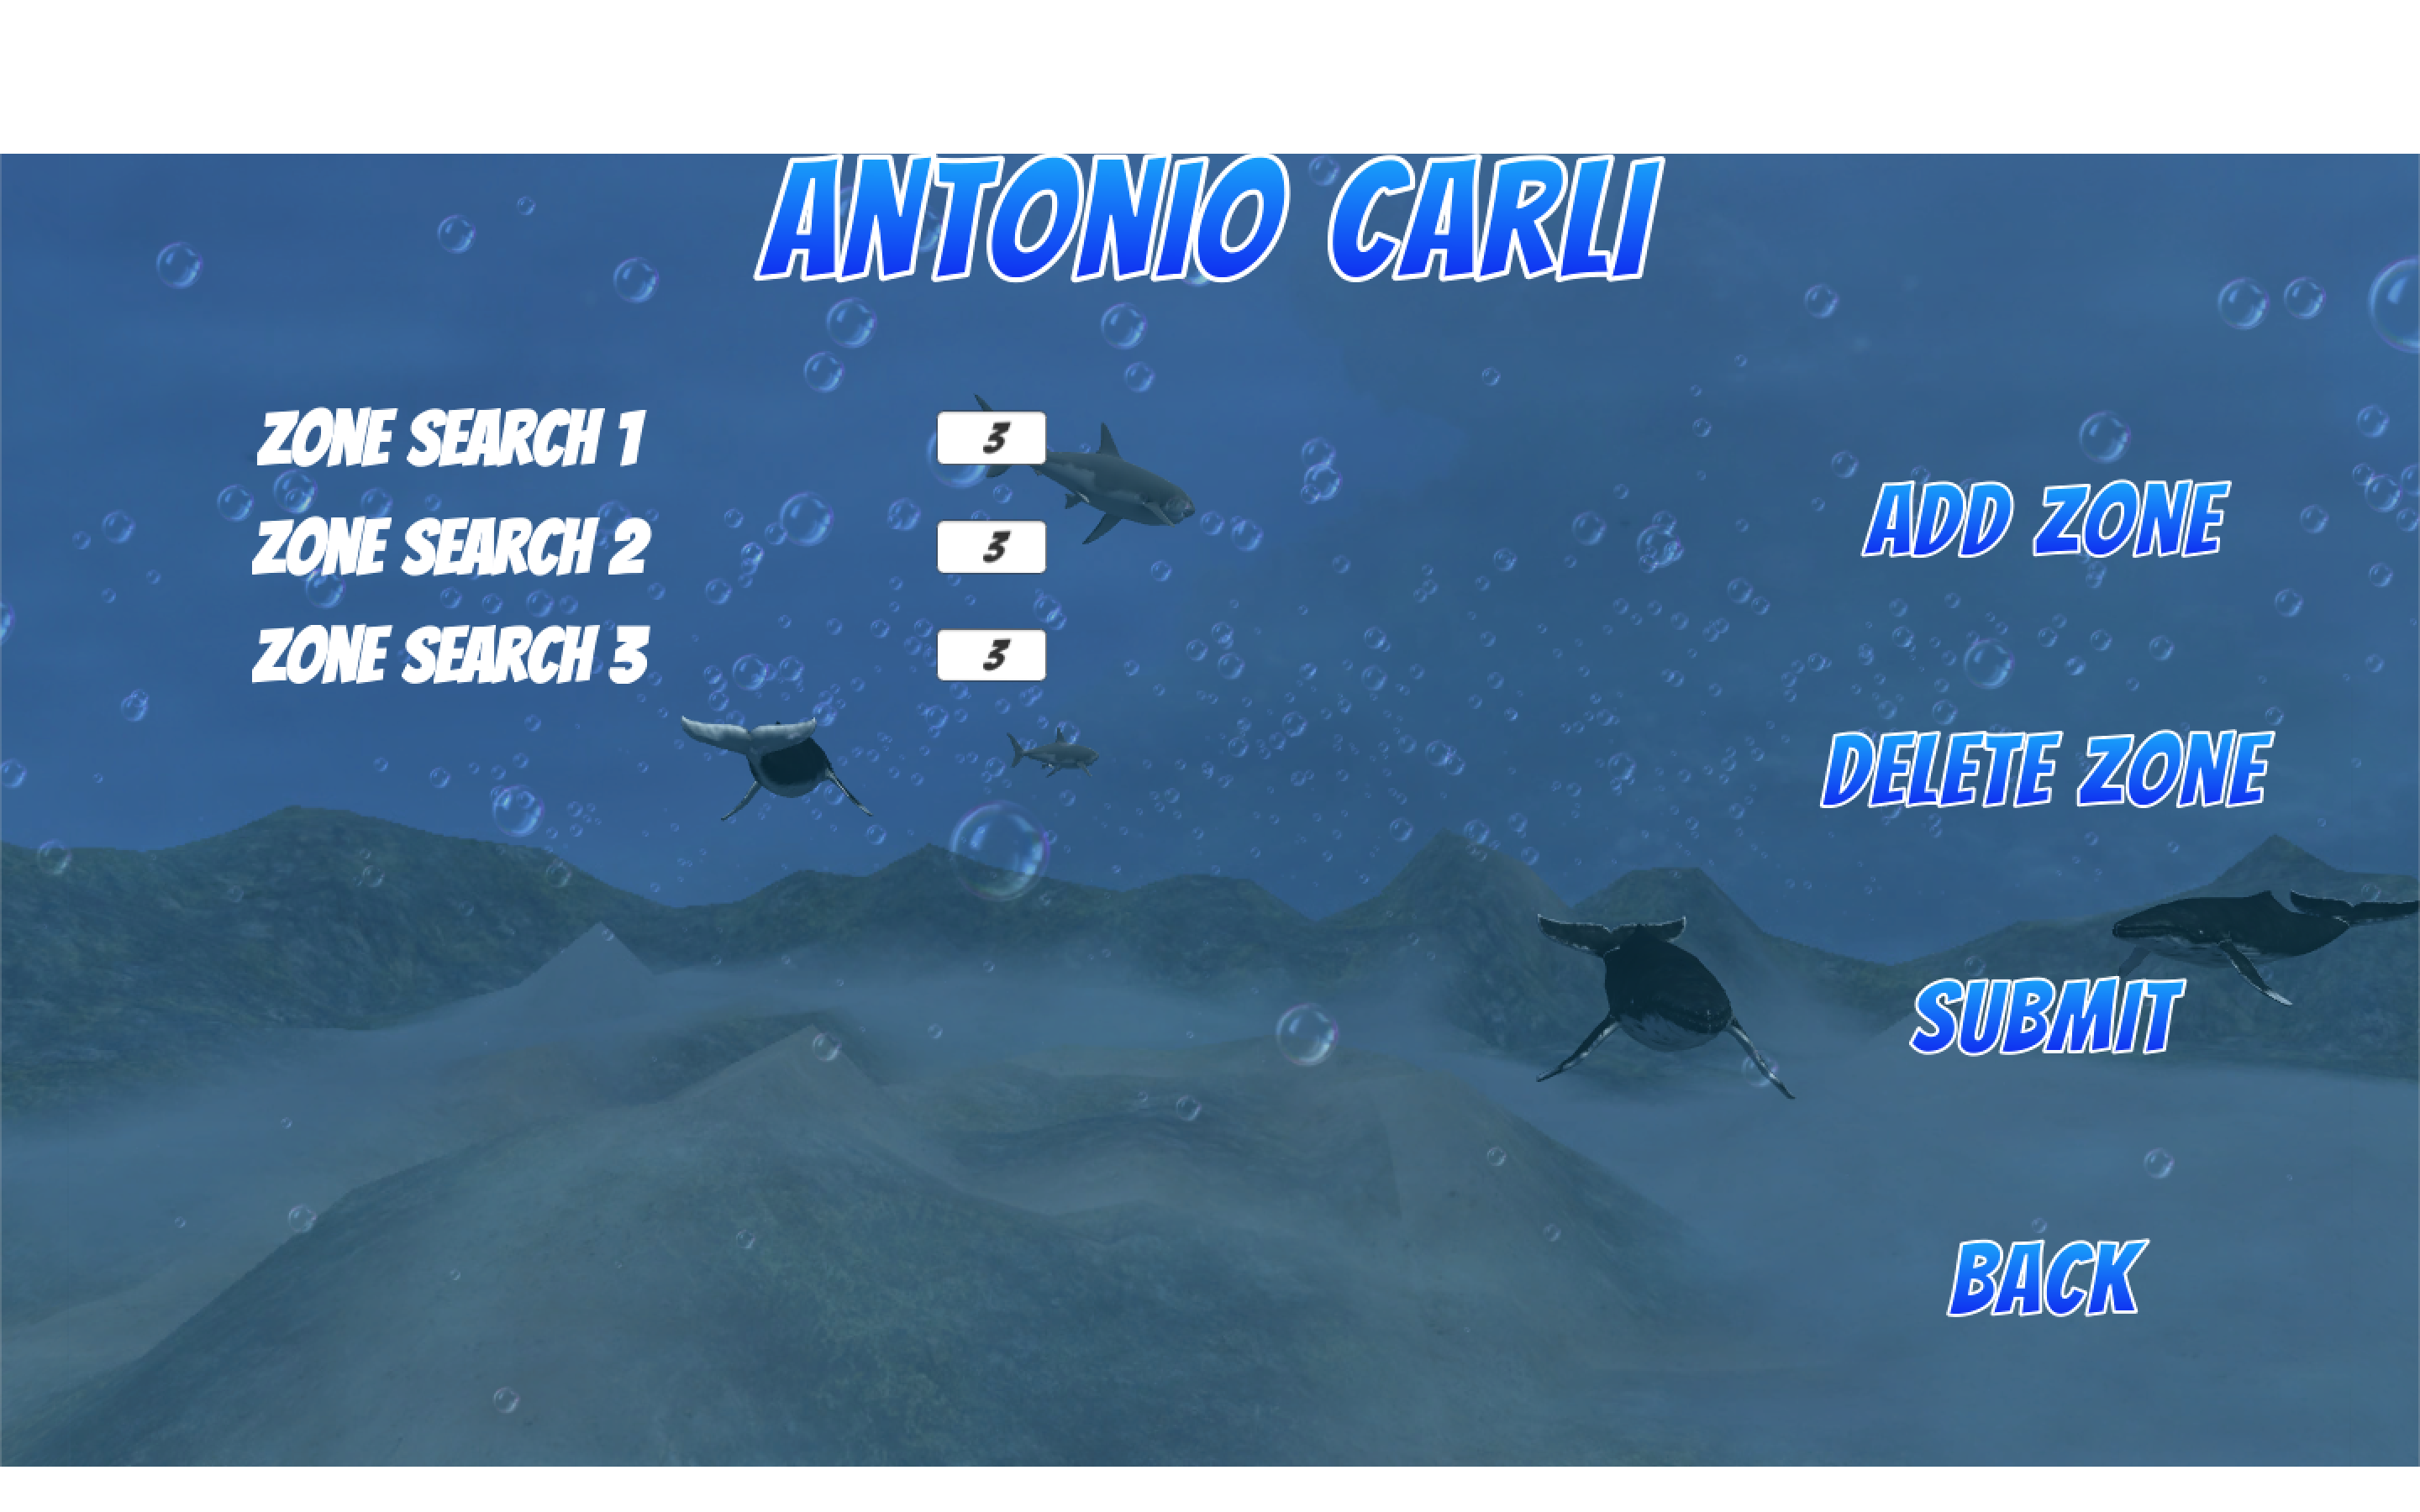
\includegraphics[width=\textwidth]{images/UX/unity/menu/5-search1}
		\caption{Parameters settings for Dolphin Run }
		\label{fig:unityParamRun}
	\end{minipage}
	\hfill
	\begin{minipage}[b]{0.4\textwidth}
		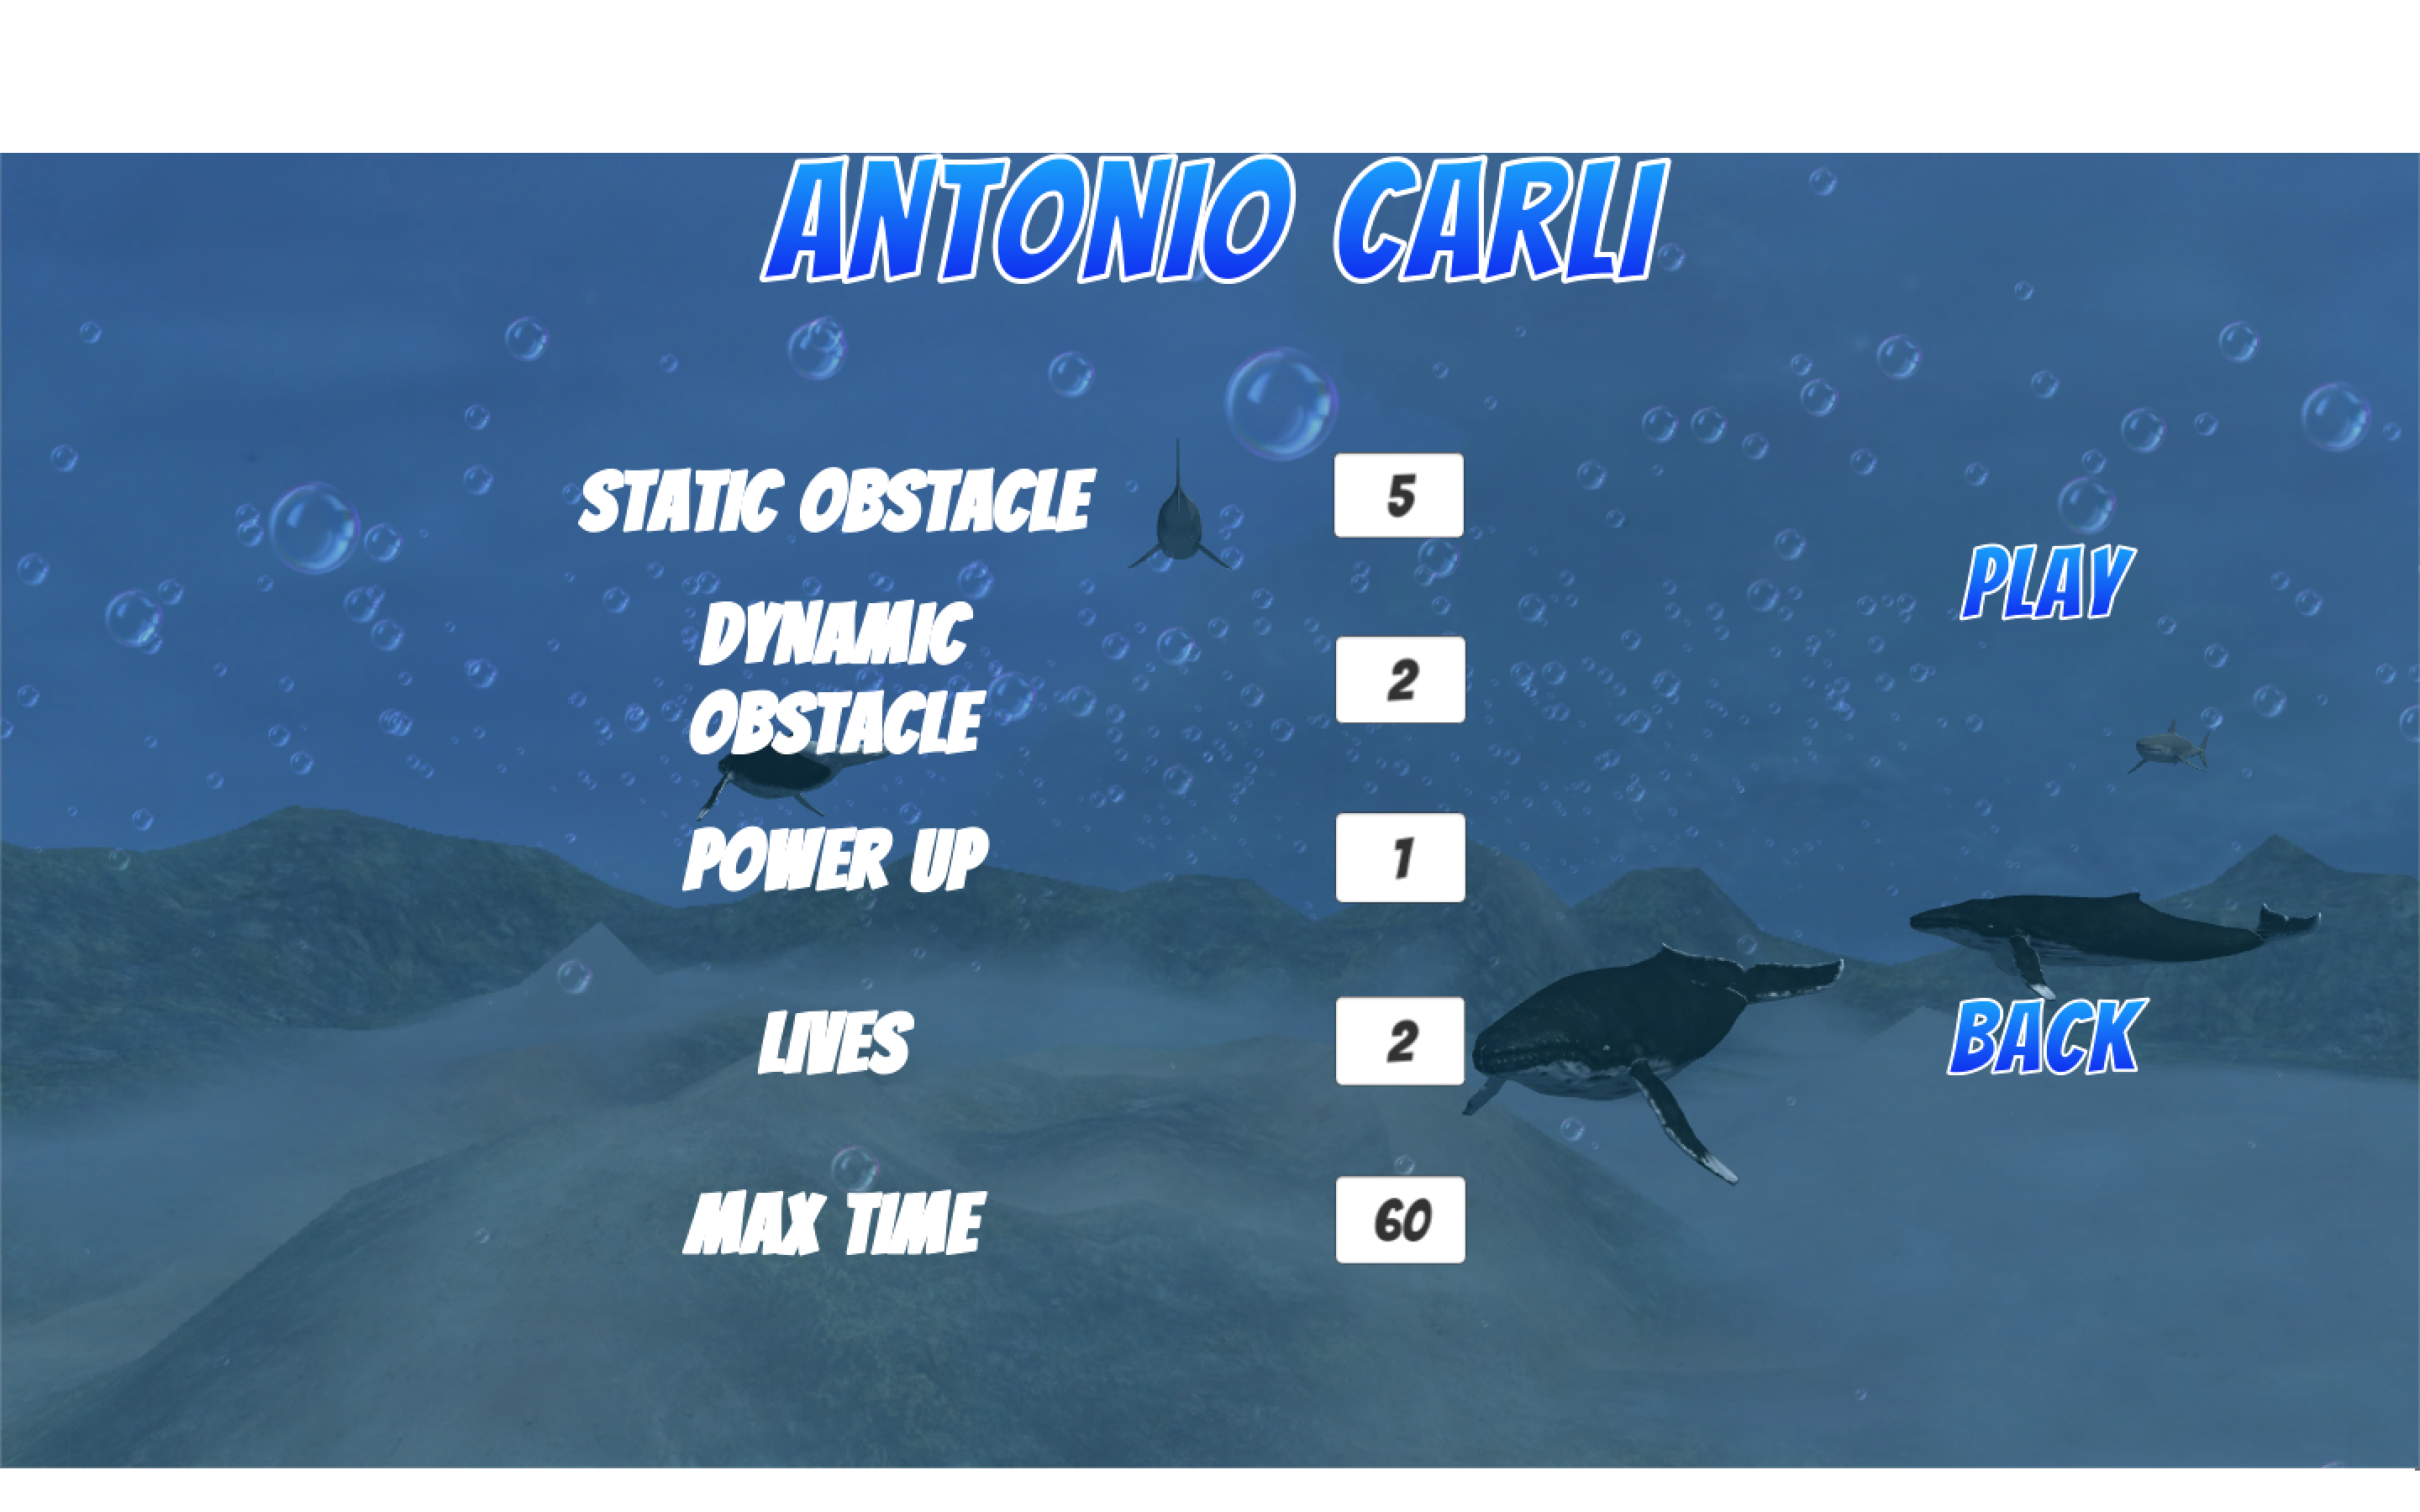
\includegraphics[width=\textwidth]{images/UX/unity/menu/8-runLevelParam}
		\caption{Parameters settings for Dolphin Search }
		\label{fig:unityParamSearch}
	\end{minipage}
\end{figure}

Depending on the selected activity then the user is redirected into the session parameters' page (Figure \ref{fig:unityParamRun}, \ref{fig:unityParamSearch}) where is possible to modify once again the patient's parameters for the next session and to store them permanently.
